% !Mode:: "TeX:UTF-8"

\chapter[基于多流语义对齐融合的开放类泛化]{基于多流语义对齐融合的开放类泛化}[]
\chaptermark{基于多流语义对齐融合的开放类泛化}
\thispagestyle{plain}
\section{引言}

跨类泛化是模型迁移研究在类别词表维度上的关键挑战，其核心要求是模型对训练阶段未见过的新颖类别保持识别能力。在密集预测任务中，这一要求体现为两个相互关联的方面：模型须为新类别给出正确的语义判别，并须在像素层面准确界定该类别的区域归属。前者要求判别依据不依附于固定类别索引，后者在训练仅覆盖有限类别时更为困难：新类别在训练阶段没有对应的像素级监督，模型倾向于将目标区域错误归入相近的已见类别。跨类泛化的研究重心，因而落在如何以多流先验的协同弥补单一语义来源在密集预测能力上的缺口。

近年来，大规模视觉—语言预训练模型在通用视觉理解任务上取得了长足进展~\cite{yin2023vlp}，其中 CLIP~\cite{radford2021learning} 与 ALIGN~\cite{jia2021scaling} 通过对比学习在海量图文对上建立了视觉与语言的联合嵌入空间，赋予模型强大的零样本泛化能力~\cite{radford2021learning,zhou2022learning}。然而，这类模型的预训练过程缺乏像素级标注，难以直接生成高质量的密集预测~\cite{rao2022denseclip}。相反，分割基础模型 SAM~\cite{kirillov2023segment} 通过大规模分割数据训练，在零样本实例分割任务上表现出色，但其本身缺乏语义理解能力。两种基础模型具有天然的互补特性：CLIP 擅长开放词汇语义识别，SAM 擅长像素级空间定位，为跨类泛化研究提供了多模态类别先验的协同来源。

现有跨类泛化方法在多流语义对齐与空间定位两个层面均存在不足。在多流语义对齐层面，现有方法主要分为两阶段与单阶段两种范式：两阶段方法~\cite{liang2023open,ding2022decoupling,xu2022simple} 通常先由额外的分割模型生成类别无关的掩码提议，再借助 ViL 模型对其进行分类，该范式存在两方面局限——掩码提议与分类过程分离导致两者所依赖的特征不对齐，且类别无关的掩码生成过程效率较低、对未见类别的掩码质量不佳；单阶段方法如 FC-CLIP~\cite{yu2023convolutions} 以 CLIP 的图像编码器为骨干端到端生成掩码提议，虽然简化了流程并缓解了提议过拟合，但其掩码质量仍受限于 CLIP 本身在像素级对齐方面的固有局限。在空间定位层面，上述方案均难以在统一解码框架内充分利用 SAM 的高质量掩码先验，致使对长尾与未见类别的细粒度识别能力受限。

上述缺陷在图~\ref{fig:cmpf_motivation} 中得到了直观体现：左图为 PC-459~\cite{mottaghi2014role} 数据集上现有 SOTA 方法 FC-CLIP 在已见与未见类别上的分割结果对比，FC-CLIP 在未见类别上的分割质量显著弱于已见类别，反映了基于 CLIP 的开放词汇分割方法对未见类别的实质性短板；右图为 CMPF 与 MaskCLIP~\cite{ding2023open}、FC-CLIP 在未见类别上的平均召回率 AR与平均交并比mIoU定量对比，进一步表明现有 CLIP 基方法在未见类别上的识别能力存在系统性不足。尽管近期工作通过类别无关掩码学习~\cite{liang2023open,dou2022learning} 与教师—学生自训练~\cite{xu2023learning} 等策略尝试缓解该问题，但均未能从根本上解决基于统一解码框架的多流语义对齐与空间定位深度融合这一核心难题。

\begin{figure}[!htbp]
    \centering
    \subfigure[]{
    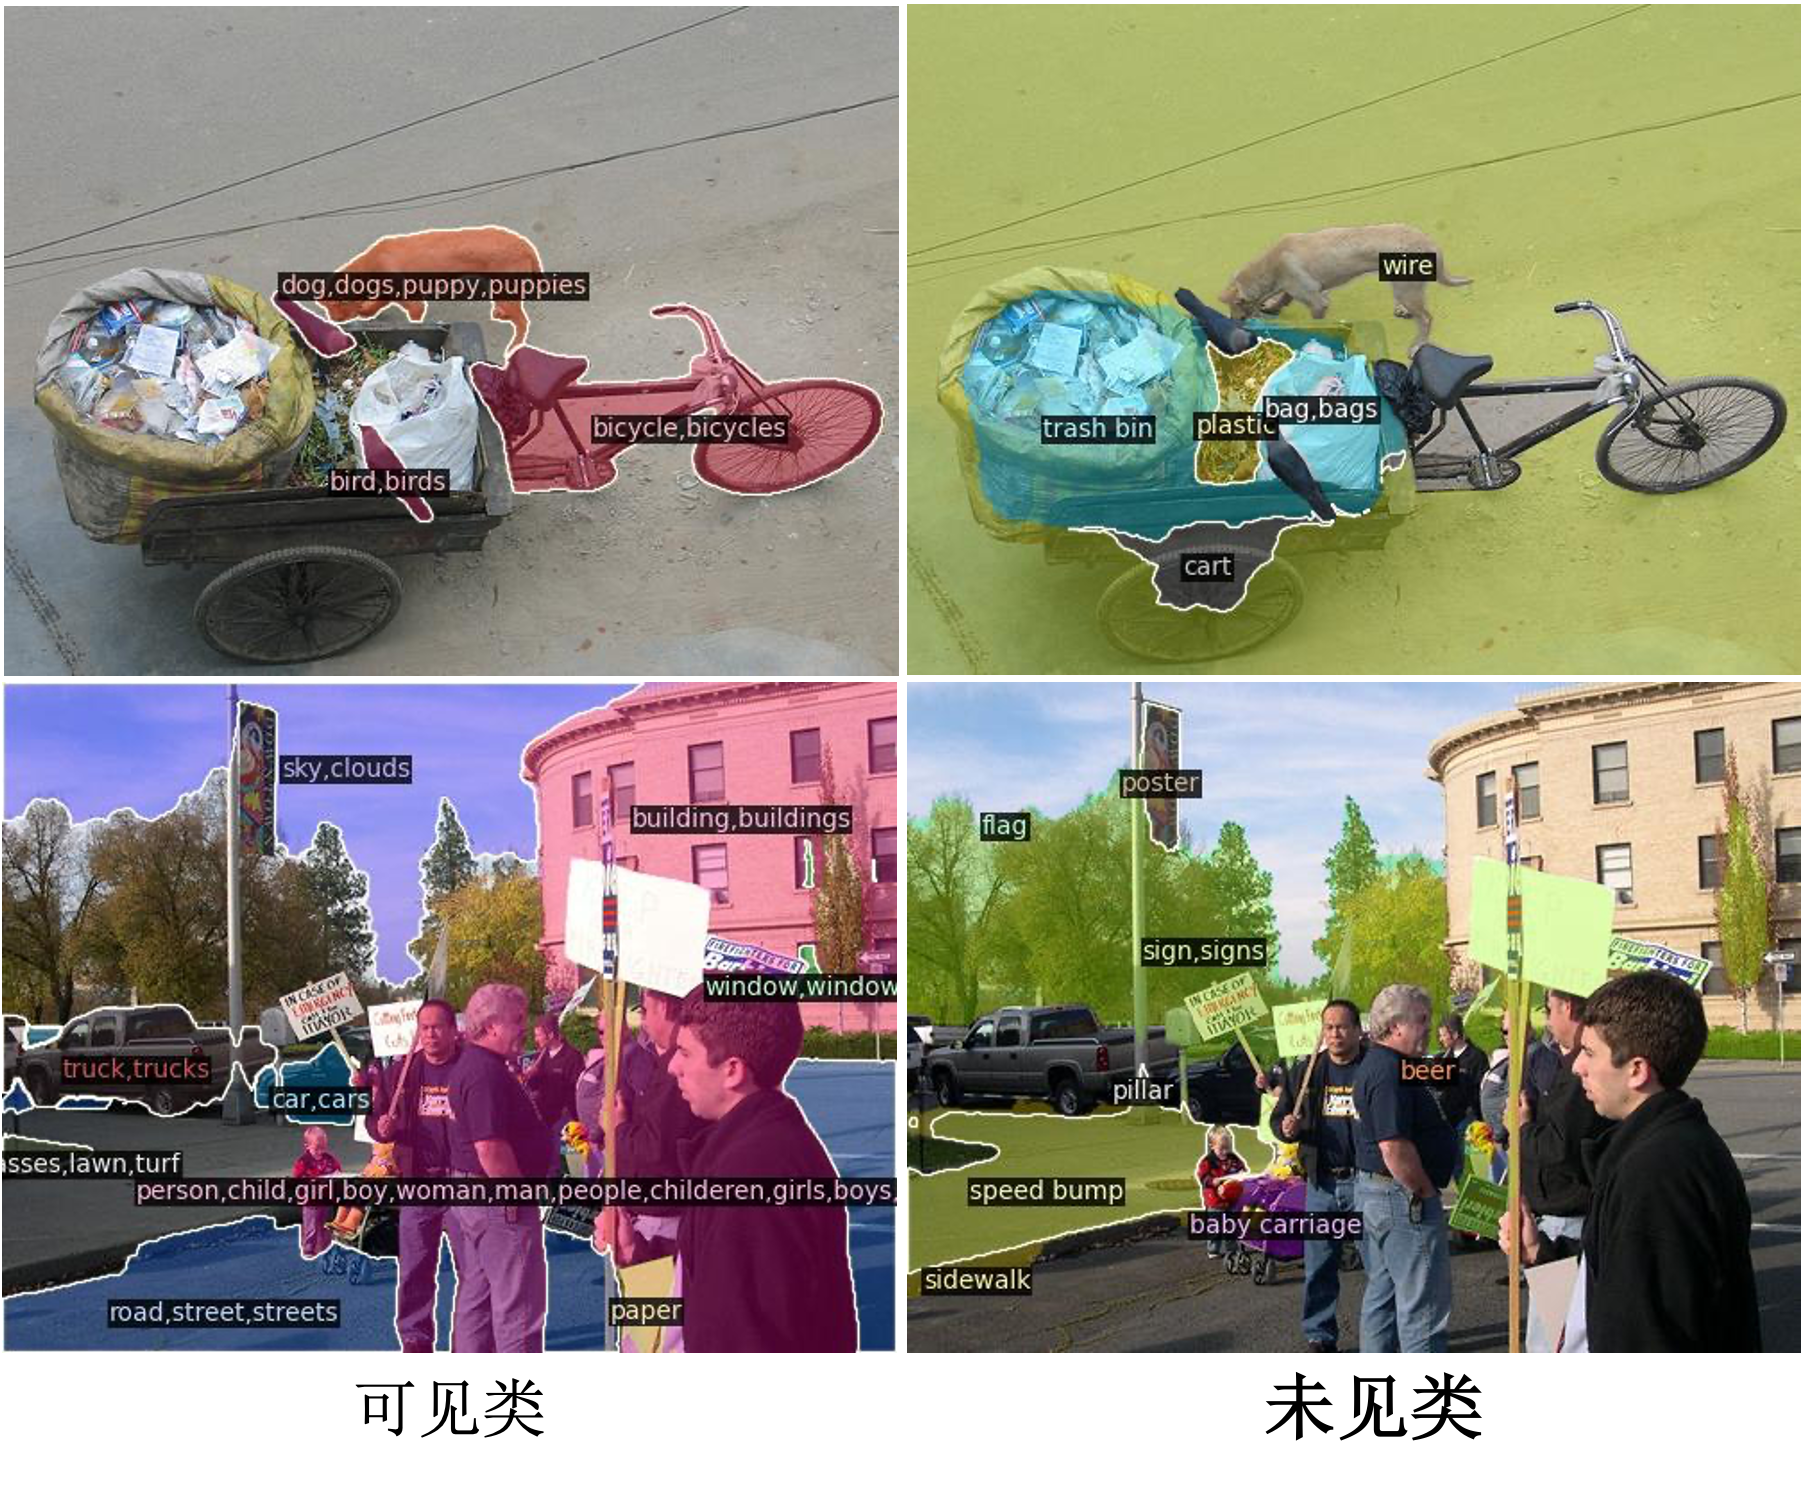
\includegraphics[width=0.58\textwidth]{figures/cmpf/moti_a.png}
    }
    \hfill
    \subfigure[]{
    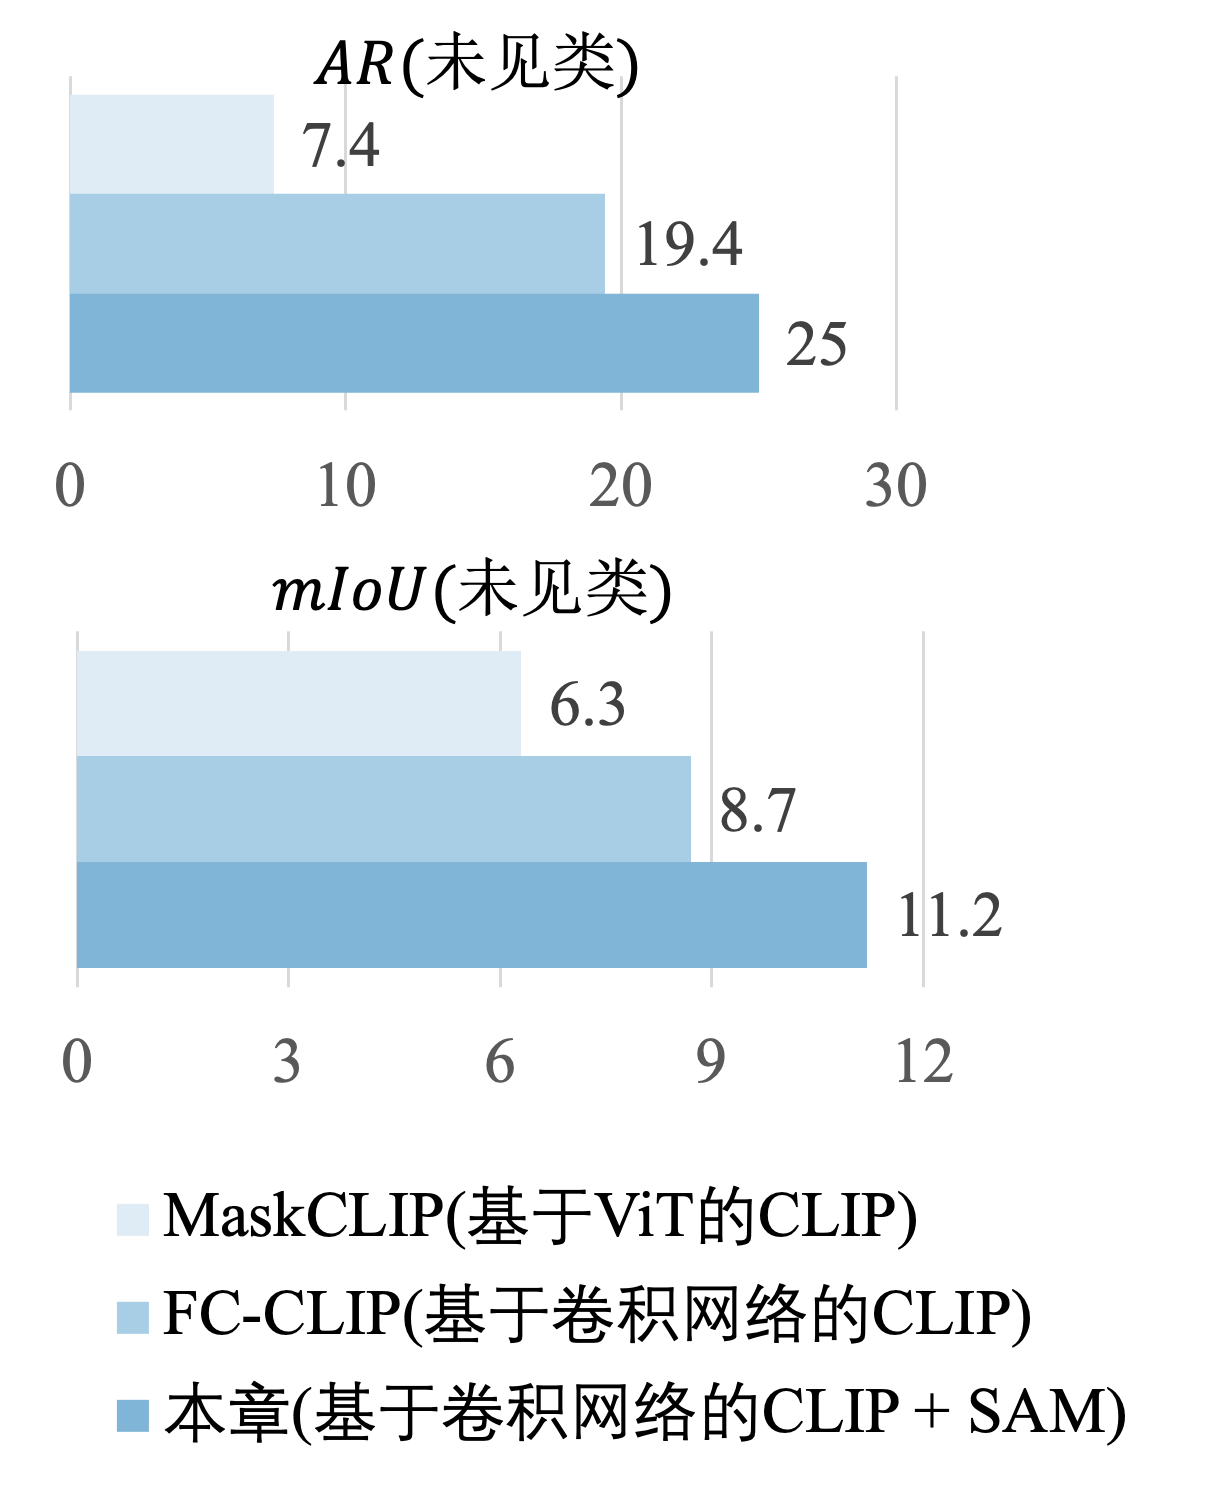
\includegraphics[width=0.38\textwidth]{figures/cmpf/moti_b.png}
    }
    \bicaption[fig:cmpf_motivation]{}{现有开放词汇SOTA方法对已见与未见类别的分割性能对比（左），及本章方法与其他两种方法的AR与mIoU对比（右）}{Fig.}{Comparison of SOTA open-vocabulary segmentation methods on seen vs unseen classes (left) and AR/mIoU on unseen classes (right) of CMPF vs MaskCLIP and FC-CLIP on PC-459}
\end{figure}

为突破上述瓶颈，本章提出基于跨模型先验融合的开放词汇分割方法 CMPF。该方法的核心思想是：协同整合SAM的像素级空间定位能力与CLIP的开放词汇语义理解能力，通过查询注入器与特征注入器两个模块在Transformer解码器内部实现两类先验知识的深度融合，并借助开放集合集成模块在推理阶段融合SAM的零样本掩码预测，进一步提升未见类别的分割质量。

本章的主要贡献可总结为以下三点：
\begin{enumerate}
    \item CMPF 跨模型先验融合框架：在 Mask2Former~\cite{cheng2021masked} 基础上首次系统性融合 SAM 的视觉定位先验与 CLIP 的语义先验，实现两类基础模型在开放词汇分割任务上的协同优化。
    \item Query Injector 与 Feature Injector：两个轻量化的注入器模块分别从查询与特征两个层面将 SAM 的细粒度空间信息注入 CLIP 驱动的解码器，在保持两个基础模型冻结的前提下提升了掩码提议质量。
    \item OpenSeg Ensemble 推理策略：通过类别集成与掩码集成两阶段融合 SAM 的零样本掩码，进一步增强对未见类别的分割泛化能力。
\end{enumerate}


\section{基于双流特征融合的开放词汇分割}

\begin{figure}[!htbp]
    \centering
    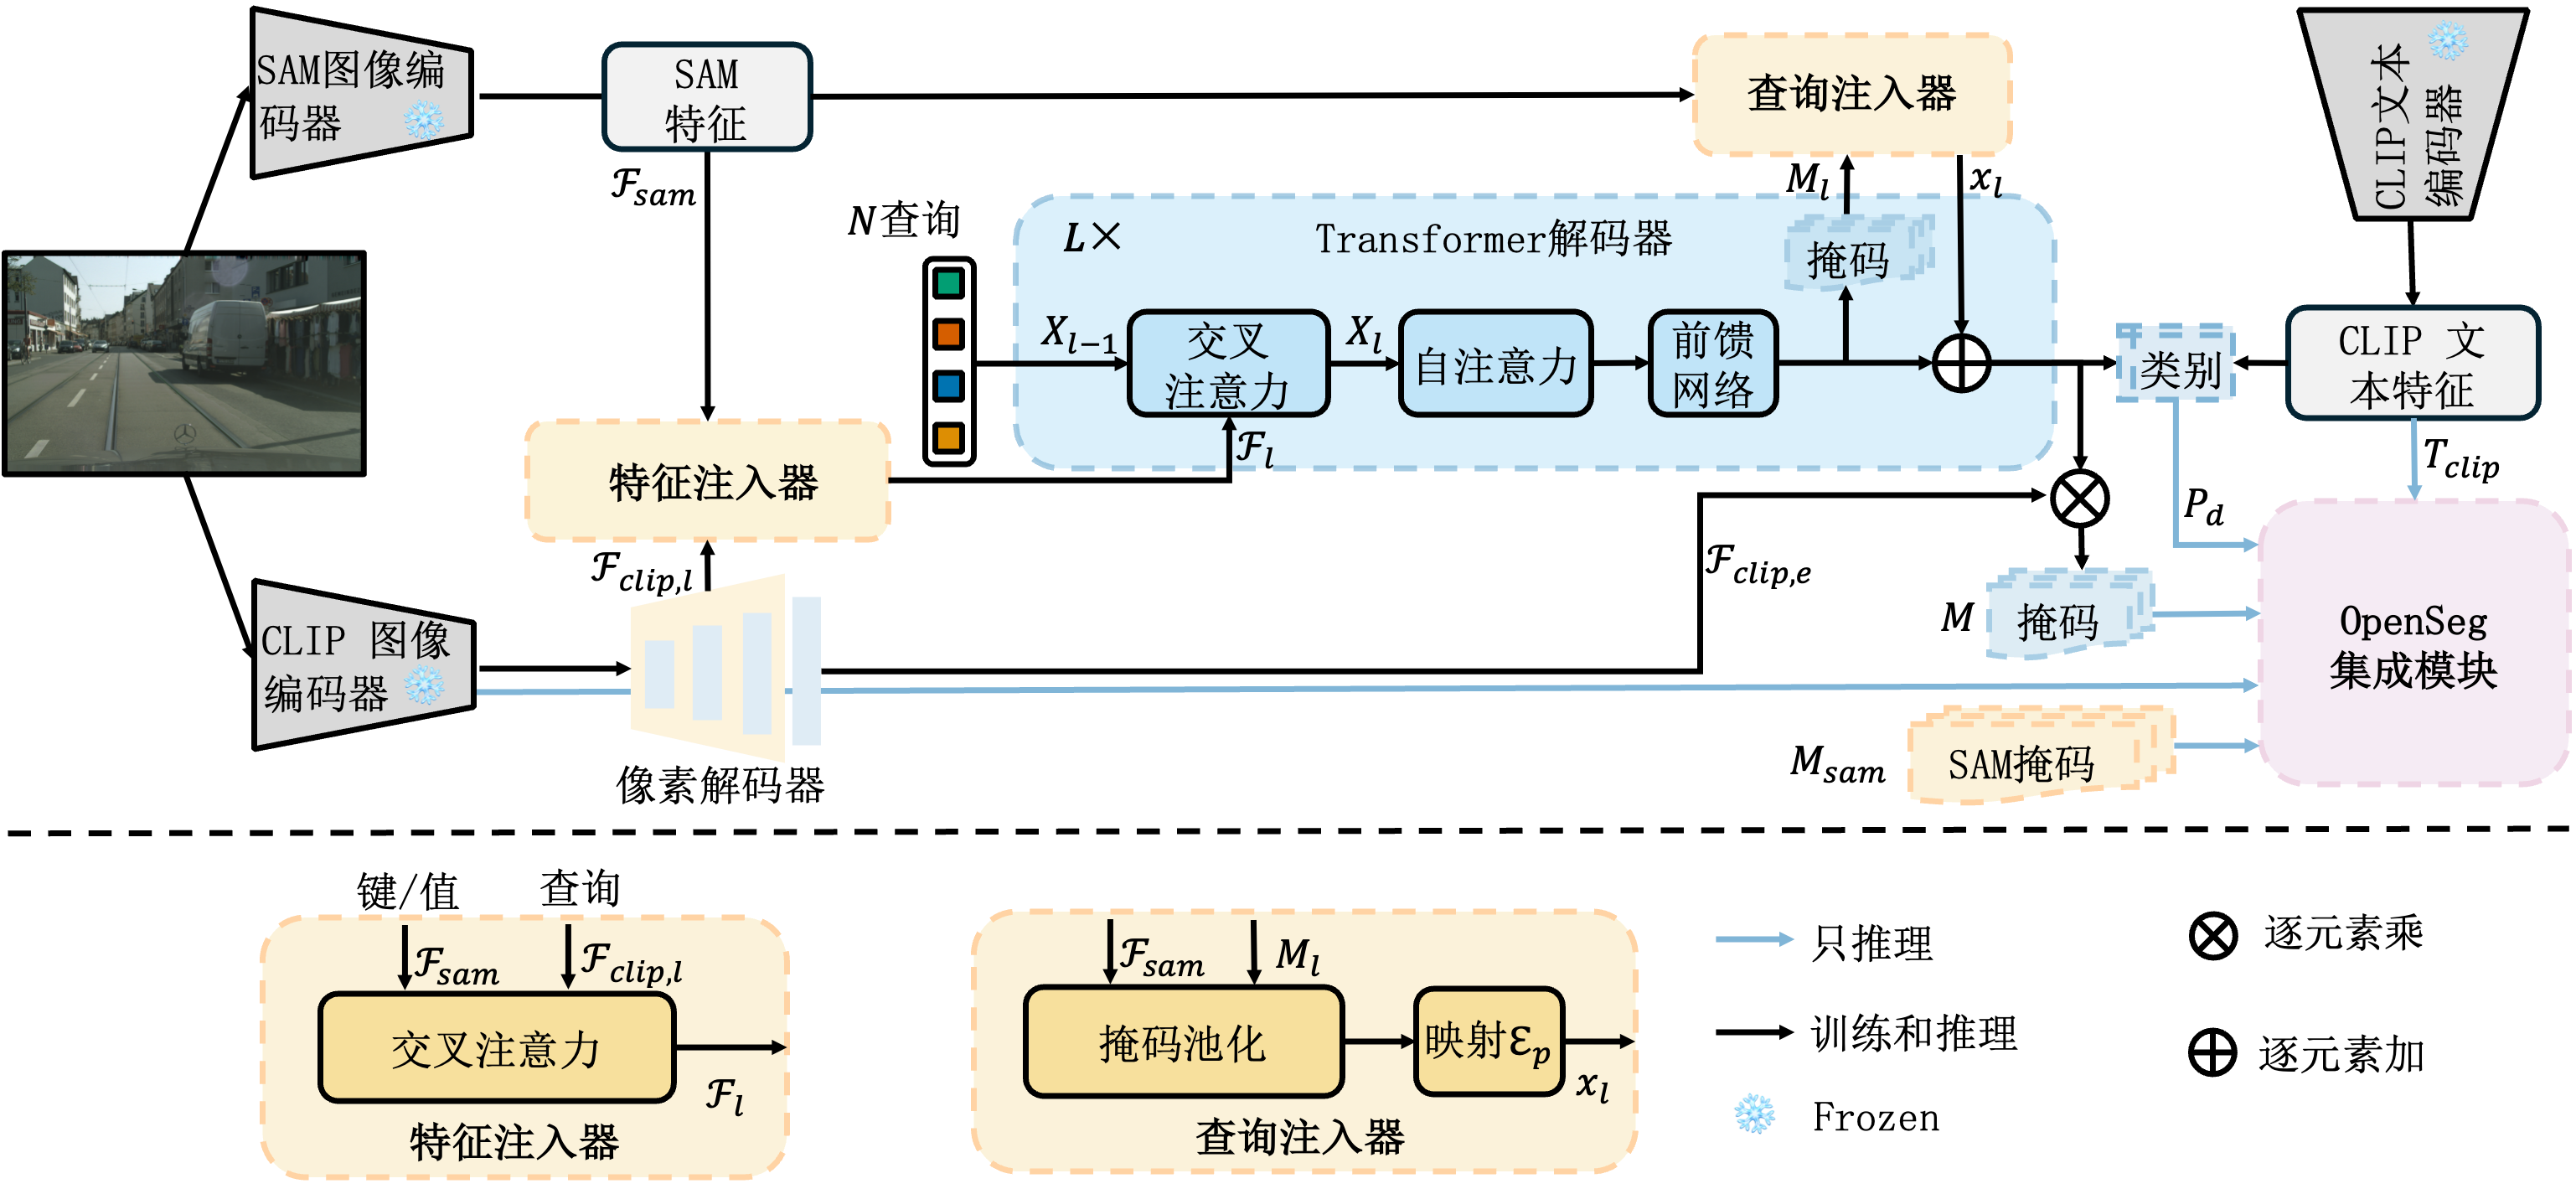
\includegraphics[width=0.95\textwidth]{figures/cmpf/frozen_framework.png}
    \bicaption[fig:cmpf_framework]{}{CMPF总体框架示意图}{Fig.}{Overview of CMPF framework}
\end{figure}

CMPF的总体框架基于Mask2Former~\cite{cheng2021masked}构建。开放词汇分割任务要求模型在训练时使用预定义类别集合 $\mathcal{C}_{\text{train}}$ 对应的真值掩码进行学习，在测试时对包含新类别的 $\mathcal{C}_{\text{test}}$ 进行零样本分割，具体可细分为语义分割（为每个像素赋予语义类别）、实例分割（识别并分割独立的目标实例）与全景分割（同时处理上述两者）。本章框架包含两个并行特征流：CLIP流与SAM流。CLIP的图像编码器作为视觉语义骨干网络，配合像素解码器生成多尺度特征$\{F_{\text{clip},l}\}_{l=1}^{L_{\text{dec}}}$与掩码特征$F_{\text{clip},e}$；SAM的图像编码器并行处理输入图像，生成细粒度空间特征$F_{\text{sam}}$。整个Transformer解码器由$L_{\text{dec}}=9$层组成，每层通过三个核心操作与图像特征交互：与特征图的交叉注意力、查询间的自注意力以及前馈网络变换。解码器维护$N_q$个可学习查询，用于生成候选掩码与类别预测。

% 为有效融合两类基础模型的互补先验，本章在解码器内部设计了两个专门的注入模块：

% \begin{itemize}
%     \item Query Injector：将SAM的细粒度空间特征通过掩码池化与投影转换为空间查询$\{x_l\}_{l=1}^{L_{\text{dec}}}$，并通过元素加法注入到Transformer解码器的可学习查询中，使查询具备空间感知能力；
%     \item Feature Injector：在CLIP特征与查询的交叉注意力之前，借助多头交叉注意力机制（MHCA）~\cite{vaswani2017attention}将SAM的空间细节与CLIP的语义特征融合，使CLIP特征在像素层面更加精细。
% \end{itemize}

% 在推理阶段，CMPF进一步引入OpenSeg Ensemble模块，通过类别集成（融合检测器与CLIP的类别预测）与掩码集成（融合SAM的零样本掩码）两阶段策略提升未见类别的分割精度。两个基础模型在整个训练与推理阶段均保持冻结，训练开销仅集中于轻量化的Transformer解码器。

\subsection{基于多尺度双注入器的掩码查询优化}

\label{sec:chap4_dual_injector}

冻结两个基础模型虽然保留了其预训练知识，但限制了模型捕获细粒度空间信息的能力。具体而言，Transformer解码器中的可学习查询仅依赖CLIP特征进行更新，缺少显式的空间锚定信号。为有效缓解这一问题，本章从查询与特征两个层面分别设计注入模块，实现SAM细粒度空间先验向CLIP驱动解码器的深度融合。

Query Injector（查询注入器）的核心思想是：将SAM的细粒度空间特征转换为空间查询，注入到解码器的查询中。给定Transformer解码器第$l$层新生成的掩码$\mathcal{M}^l$，Query Injector通过掩码池化在SAM特征$F_{\text{sam}}$上提取与当前掩码区域对齐的空间特征，并经过投影函数$E_p$转换为空间查询：
\begin{equation}
x^l = E_p(\mathrm{pool}_{\mathcal{M}^l} F_{\mathrm{sam}}).
\label{eq:query_injector}
\end{equation}

该空间查询专注于掩码所覆盖的前景区域，与可学习查询$X^l$进行元素加法后送入下一解码器层：
\begin{equation}
X^l_{\text{enhanced}} = X^l + x^l.
\end{equation}

这种设计带来两方面优势：（1）空间查询为解码器提供了显式的像素级空间锚定，使查询能够“知道”自己应该关注图像中的哪个区域；（2）注入位置设计为解码器中间层（$l=3,6,9$），既保证查询有足够的时间与CLIP特征进行多轮语义交互，又使后续的解码层能够对新引入的空间信息进行进一步精炼。

Feature Injector（特征注入器）从特征层面进一步提升CLIP的像素级表征能力。该模块借助多头交叉注意力（MHCA）~\cite{vaswani2017attention}机制，在解码器与CLIP特征进行交叉注意力之前，将SAM的空间细节显式地融合到CLIP的图像特征中。Feature Injector首先对CLIP特征进行查询、对SAM特征进行键值投影，然后通过注意力计算生成增强后的CLIP特征：
\begin{equation}
F^l = \mathrm{Softmax}\bigg(\frac{f_q(F_{\mathrm{clip},l})f_k(F_{\mathrm{sam}})^\top}{\sqrt{d_k}}\bigg) f_v(F_{\mathrm{sam}})，
\label{eq:feature_injector}
\end{equation}
其中$f_q$、$f_k$、$f_v$为MHCA的线性投影函数，$\sqrt{d_k}$为缩放因子。为控制计算复杂度，Feature Injector仅在低分辨率特征（$1/32$尺度）上应用，对应解码器的层$l=1,4,7$。

在解码器每一层$l$，模型通过三个投影函数完成预测：（1）$E_m$将查询特征投影为掩码预测的查询嵌入；（2）$E_{aux}$将池化后的掩码特征投影为预测辅助嵌入；（3）$E_c$将查询特征投影为CLIP文本对齐的类别嵌入。掩码预测通过查询嵌入与CLIP掩码特征的乘积生成：
\begin{equation}
\mathcal{M}^l = E_m(X^l) \cdot F_{\mathrm{clip},e},
\label{eq:mask_pred}
\end{equation}
其中$\mathcal{M}^l$为连续掩码值，最终层输出记为$\mathcal{M}=\{m_i\}_{i=1}^{N_q}$。类别预测则通过类别嵌入与CLIP文本特征$T_{\mathrm{clip}}$的对齐计算：
\begin{equation}
P_d = \mathrm{Softmax}\big(E_c(X^l + E_{aux}(\mathrm{pool}_{\mathcal{M}} F_{\mathrm{clip},e})) \cdot T_{\mathrm{clip}}^\top / \tau\big),
\label{eq:class_pred}
\end{equation}
其中$\tau$为可学习的温度参数。解码器采用Masked Attention机制：每层交叉注意力的掩码$\mathcal{M}^{l-1}$由前一层预测计算：
\begin{equation}
\mathcal{M}^{l-1}_{[x,y]} = \begin{cases} 0, & \mathcal{M}^{l-1}_{[x,y]} > 0, \\ -\infty, & \text{otherwise}, \end{cases}
\label{eq:mask_attn}
\end{equation}
使注意力计算聚焦于预测的前景区域。

\subsection{基于零样本掩码集成的分割推理优化}

\label{sec:chap4_openseg_ensemble}

为充分利用SAM的零样本分割能力，CMPF在推理阶段引入OpenSeg Ensemble模块。该模块通过两阶段融合策略，将解码器输出与SAM的零样本掩码预测进行深度融合。如图~\ref{fig:openseg_ensemble}所示，OpenSeg Ensemble首先在输入图像上均匀采样$32\times 32$个点作为SAM的提示，生成类别无关掩码$\mathcal{M}_{\mathrm{sam}}$，然后通过两阶段融合提升分割精度。

\begin{figure}[!htbp]
    \centering
    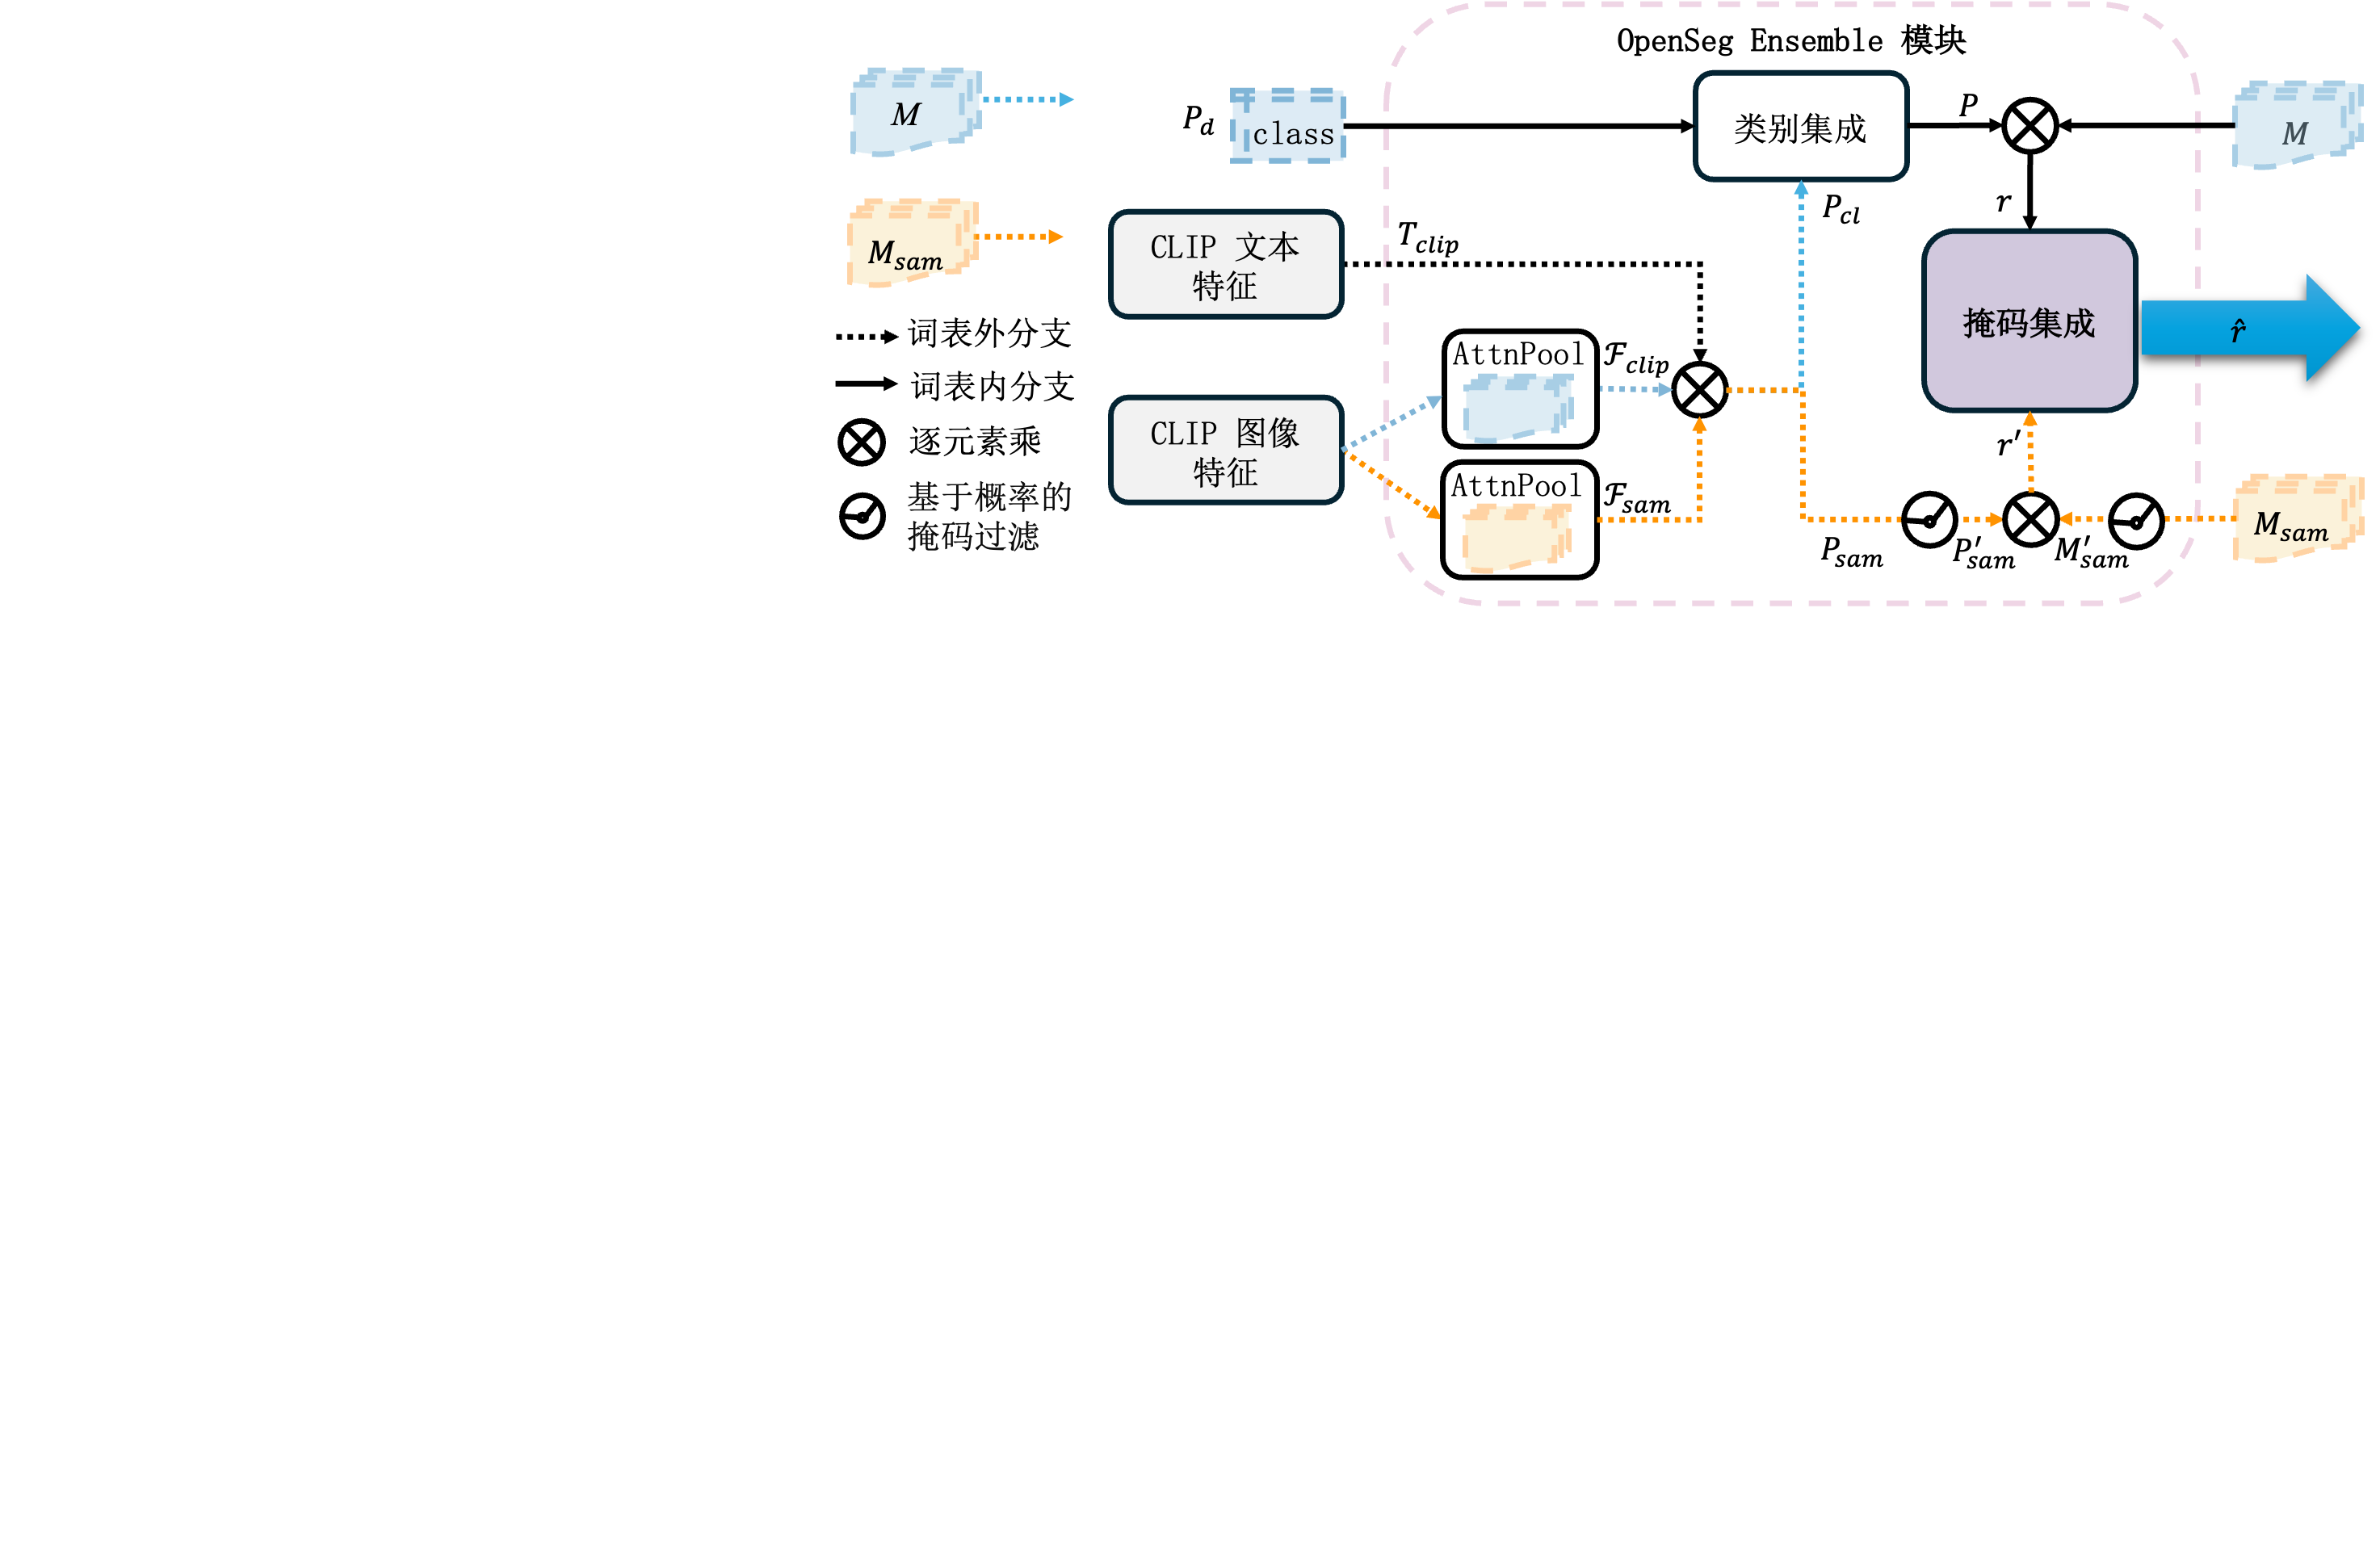
\includegraphics[width=0.95\textwidth]{figures/cmpf/maskEnsemble.png}
    \bicaption[fig:openseg_ensemble]{}{OpenSeg Ensemble模块结构示意图}{Fig.}{Architecture of the OpenSeg Ensemble Module}
\end{figure}


首先类别集成的目标是将检测器预测与CLIP直接预测进行有效融合。给定检测器预测$P_d=\{p_{i,d}\}_{i=1}^{N_q}$与基于掩码池化CLIP特征的CLIP预测$P_{\mathrm{cl}}=\{p_{i,\mathrm{cl}}\}_{i=1}^{N_q}$，类别集成通过加权几何平均计算融合后的类别概率：
\begin{equation}
p_i(j) = \begin{cases} (p_{i,d}(j))^{1-\alpha_{\text{ens}}} \cdot (p_{i,\mathrm{cl}}(j))^{\alpha_{\text{ens}}}, & j \in \mathcal{C}_{\text{train}}, \\ (p_{i,d}(j))^{1-\beta_{\text{ens}}} \cdot (p_{i,\mathrm{cl}}(j))^{\beta_{\text{ens}}}, & \text{otherwise}, \end{cases}
\label{eq:class_ensemble}
\end{equation}
其中$\alpha_{\text{ens}}=0.4$，$\beta_{\text{ens}}=0.8$为平衡系数。$P_{\mathrm{cl}}$通过在掩码区域上对CLIP图像特征进行AttnPool池化后与文本特征对齐得到。
类别集成得到的概率-掩码对$(P, \mathcal{M})$被用于生成初步的语义分割结果$r = \sum_{i=1}^{N_q} p_i(c) \cdot m_{i,[x,y]}$。

掩码集成进一步引入SAM的零样本掩码预测。具体地，首先对$\mathcal{M}_{\mathrm{sam}}$应用AttnPool得到SAM-CLIP特征并计算类别分数$P_{\mathrm{sam}}$，使用阈值$\xi=0.5$过滤低质量掩码，得到选中的概率-掩码对$(\mathcal{M}'_{\mathrm{sam}}, P'_{\mathrm{sam}})$。

最终的语义分割结果$\hat{r}$通过两路预测的加权融合得到：
\begin{equation}
\hat{r}_{[x,y]}(j) = \begin{cases} r_{[x,y]}(j), & j \in \mathcal{C}_{\text{train}}, \\ (1-\epsilon_{\text{fuse}}) r_{[x,y]}(j) + \epsilon_{\text{fuse}} r'_{[x,y]}(j), & \text{otherwise}, \end{cases}
\label{eq:mask_ensemble}
\end{equation}
其中$\epsilon_{\text{fuse}}=0.2$控制SAM零样本掩码在未见类别上的融合权重。该设计使SAM的零样本分割能力专门用于提升未见类别的识别精度，而对训练集内的类别则保持原有检测器的预测，避免引入SAM的分割噪声。

在全景分割任务中，由于最终结果依赖单个查询的预测质量，集成更多含噪SAM掩码反而可能降低精度，因此仅采用类别集成而不进行掩码集成。

\section{实验结果与分析}

\noindent\textbf{(1)数据集与实验设置}

模型仅在COCO Panoptic~\cite{lin2014microsoft}数据集上进行训练，该数据集包含133个类别。遵循零样本评估协议，模型在全景分割的ADE20K~\cite{zhou2017scene}、Cityscapes~\cite{cordts2016cityscapes}、BDD100K~\cite{yu2020bdd100k}三个基准上测试，使用PQ、AP、mIoU作为评价指标；在语义分割的PASCAL-Context（PC-459与PC-59）~\cite{mottaghi2014role}、ADE20K（A-847与A-150）两个基准上测试，使用mIoU作为评价指标；在实例分割的LVIS v1.0~\cite{gupta2019lvis}基准上测试，以rare类别的$\mathrm{AP}_r$作为主要评价指标。

实验采用RN50$\times$64与ConvNeXt-Large两种规模的CLIP图像编码器，以及ViT-Base的SAM图像编码器（基于消融分析的最优选择）。Transformer解码器层数$L_{\text{dec}}=9$，特征分辨率为$1/8$、$1/16$、$1/32$循环处理。Query Injector在第$3,6,9$层注入，Feature Injector在第$1,4,7$层应用。训练数据流为COCO Panoptic，4卡Tesla A100 GPU，batch size=16。推理时输入图像最短边resize到800像素（Cityscapes为1024），OpenSeg Ensemble默认参数$\alpha_{\text{ens}}=0.4$、$\beta_{\text{ens}}=0.8$、$\epsilon_{\text{fuse}}=0.2$，SAM使用ViT-Huge，$32\times 32$均匀采样点提示，独立生成类别无关的零样本掩码，并将其与解码器输出在未见类别上做加权融合。该阶段直接消费的是SAM输出的掩码质量本身，因此推理阶段改用规模更大的ViT-Huge。


\noindent\textbf{(2)实验结果和分析}

表~\ref{tab:panoptic_cmpf}给出了在ADE20K、Cityscapes与BDD100K三个数据集上的开放词汇全景分割结果。CMPF在所有数据集与骨干设置下均取得最优性能：在RN50$\times$64骨干下，全景分割指标较FC-CLIP有稳定的提升，在BDD100K上的差距相对更大。切换至ConvNeXt-L骨干后，三个数据集的全景分割指标进一步提升，说明跨模型先验融合策略的收益不依赖于特定骨干规模。
图~\ref{fig:cmpf_moti}与图~\ref{fig:cmpf_bdd}分别给出了Cityscapes与BDD100K上的全景分割可视化对比。可视化结果印证了定量分析：相较于FC-CLIP，CMPF在未见类别（如Cityscapes中的“rider”、BDD100K中的“vegetation”与“street light”）上展现出更强的泛化能力，同时对小目标的检测精度与独立实例的识别准确度也有明显改善。

\begin{table*}[!htbp]\centering
    \bicaption[tab:panoptic_cmpf]{}{开放词汇全景分割结果对比}{Table}{Open-vocabulary panoptic segmentation results}
    % \setlength{\tabcolsep}{1pt}
    \vspace{0.5em}\centering\wuhao
    % \resizebox{.8\textwidth}{!}{
    \begin{tabular}{lccccccccc}
        \toprule
        \multirow{2}{*}{方法} & \multirow{2}{*}{ViL Model} & \multicolumn{3}{c}{ADE20K} & \multicolumn{3}{c}{Cityscapes} & \multicolumn{2}{c}{BDD100K} \\
        \cline{3-10}
         &       & PQ & AP & mIoU & PQ & AP & mIoU & PQ & mIoU \\
        \midrule
        OPSNet~\cite{chen2023open}    & RN50        & 19.0 & --   & 25.4 & 41.5 & --   & --   & --   & --   \\
        MaskCLIP~\cite{ding2023open}  & ViT-L/14    & 15.1 & 6.0  & 23.7 & --   & --   & --   & --   & --   \\
        MasQCLIP~\cite{MasQCLIP} & ViT-L/14    & 23.3 & --   & 30.4 & --   & --   & --   & --   & --   \\
        ODISE~\cite{xu2023open}        & ViT-L/14    & 22.6 & 14.4 & 29.9 & --   & --   & --   & --   & --   \\
        ODISE+CLIPSelf~\cite{wu2024clipself} & ViT-L/14 & 23.7 & 13.6 & 30.1 & -- & -- & -- & -- & -- \\
        \midrule
        FC-CLIP~\cite{yu2023convolutions} & RN50$\times$64 & 21.3 & 13.2 & 28.7 & 42.6 & 27.3 & 55.1 & 13.8 & 41.4 \\
        \textbf{CMPF}                & RN50$\times$64 & \textbf{23.1} & \textbf{13.5} & \textbf{30.7} & \textbf{45.2} & \textbf{28.9} & \textbf{56.0} & \textbf{12.9} & \textbf{46.2} \\
        \midrule
        FC-CLIP~\cite{yu2023convolutions} & ConvNeXt-L & 25.1 & 16.4 & 32.8 & 44.3 & 27.9 & 56.0 & 17.9 & 49.4 \\
        EOV-Seg~\cite{niu2025eov}     & ConvNeXt-L  & 24.5 & 13.7 & 32.1 & --   & --   & --   & --   & --   \\
        \textbf{CMPF}                & ConvNeXt-L  & \textbf{25.9} & \textbf{16.5} & \textbf{34.4} & \textbf{45.8} & \textbf{28.4} & \textbf{56.8} & \textbf{19.3} & \textbf{52.3} \\
        \bottomrule
    \end{tabular}
    % }
\end{table*}


\begin{figure}[!htbp]
    \centering
    \subfigure[]{
    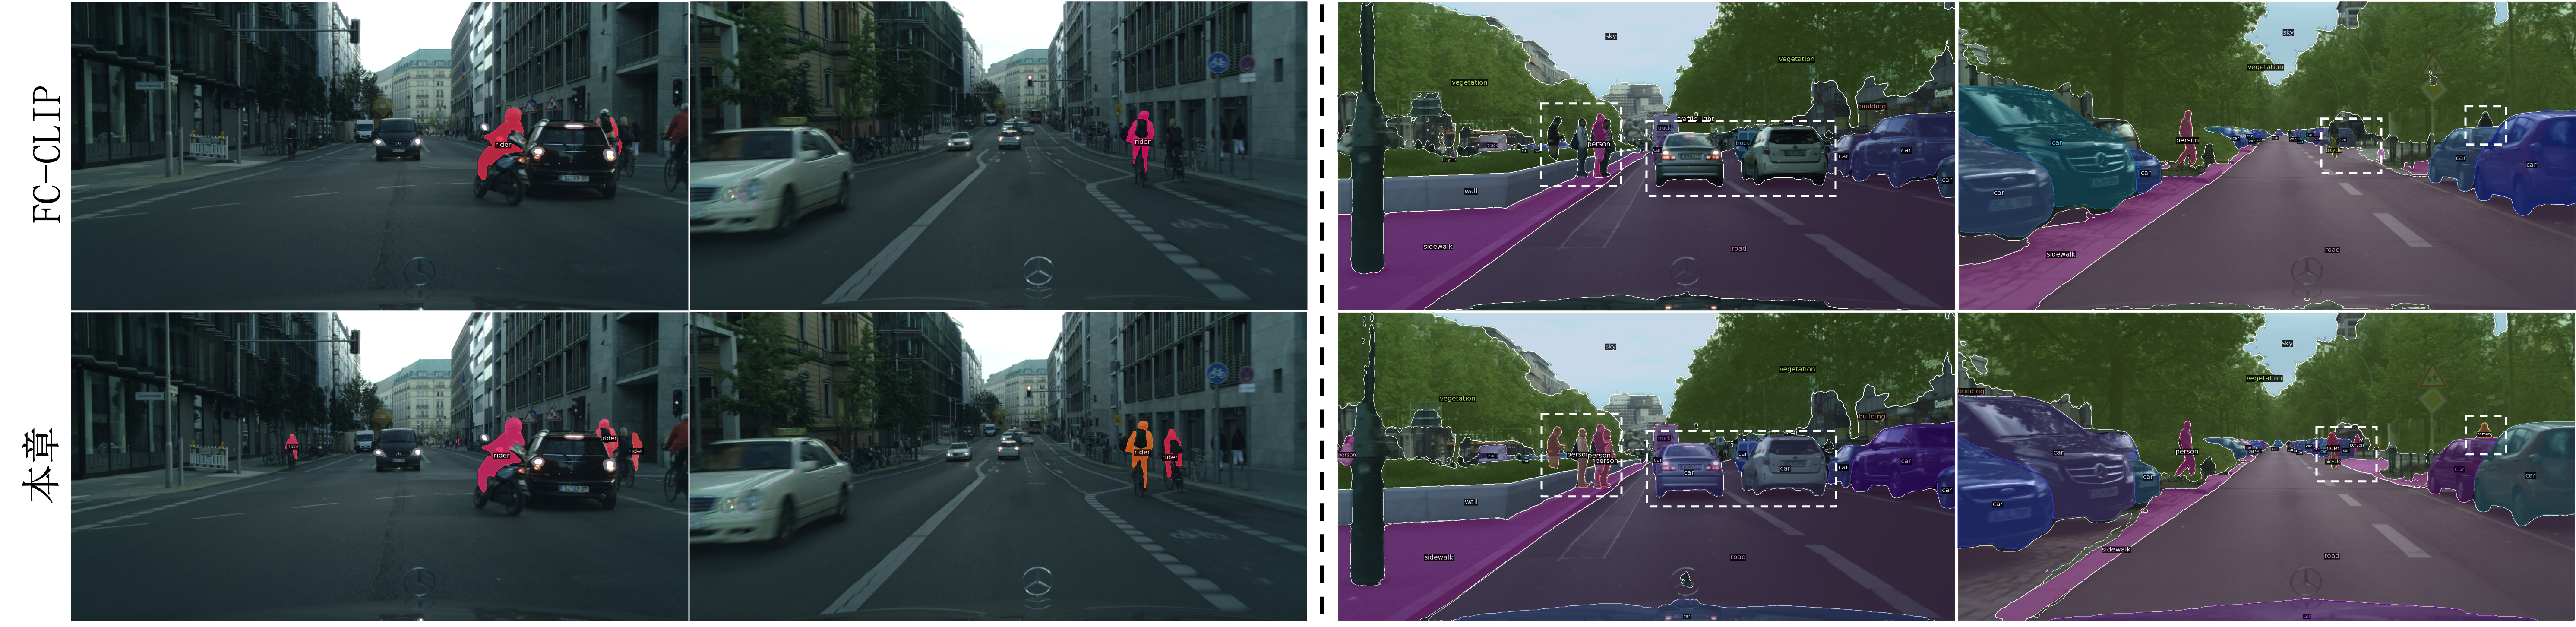
\includegraphics[width=1.\linewidth]{figures/cmpf/panop_city.png}
    \label{fig:cmpf_moti}
    }
    \subfigure[]{
    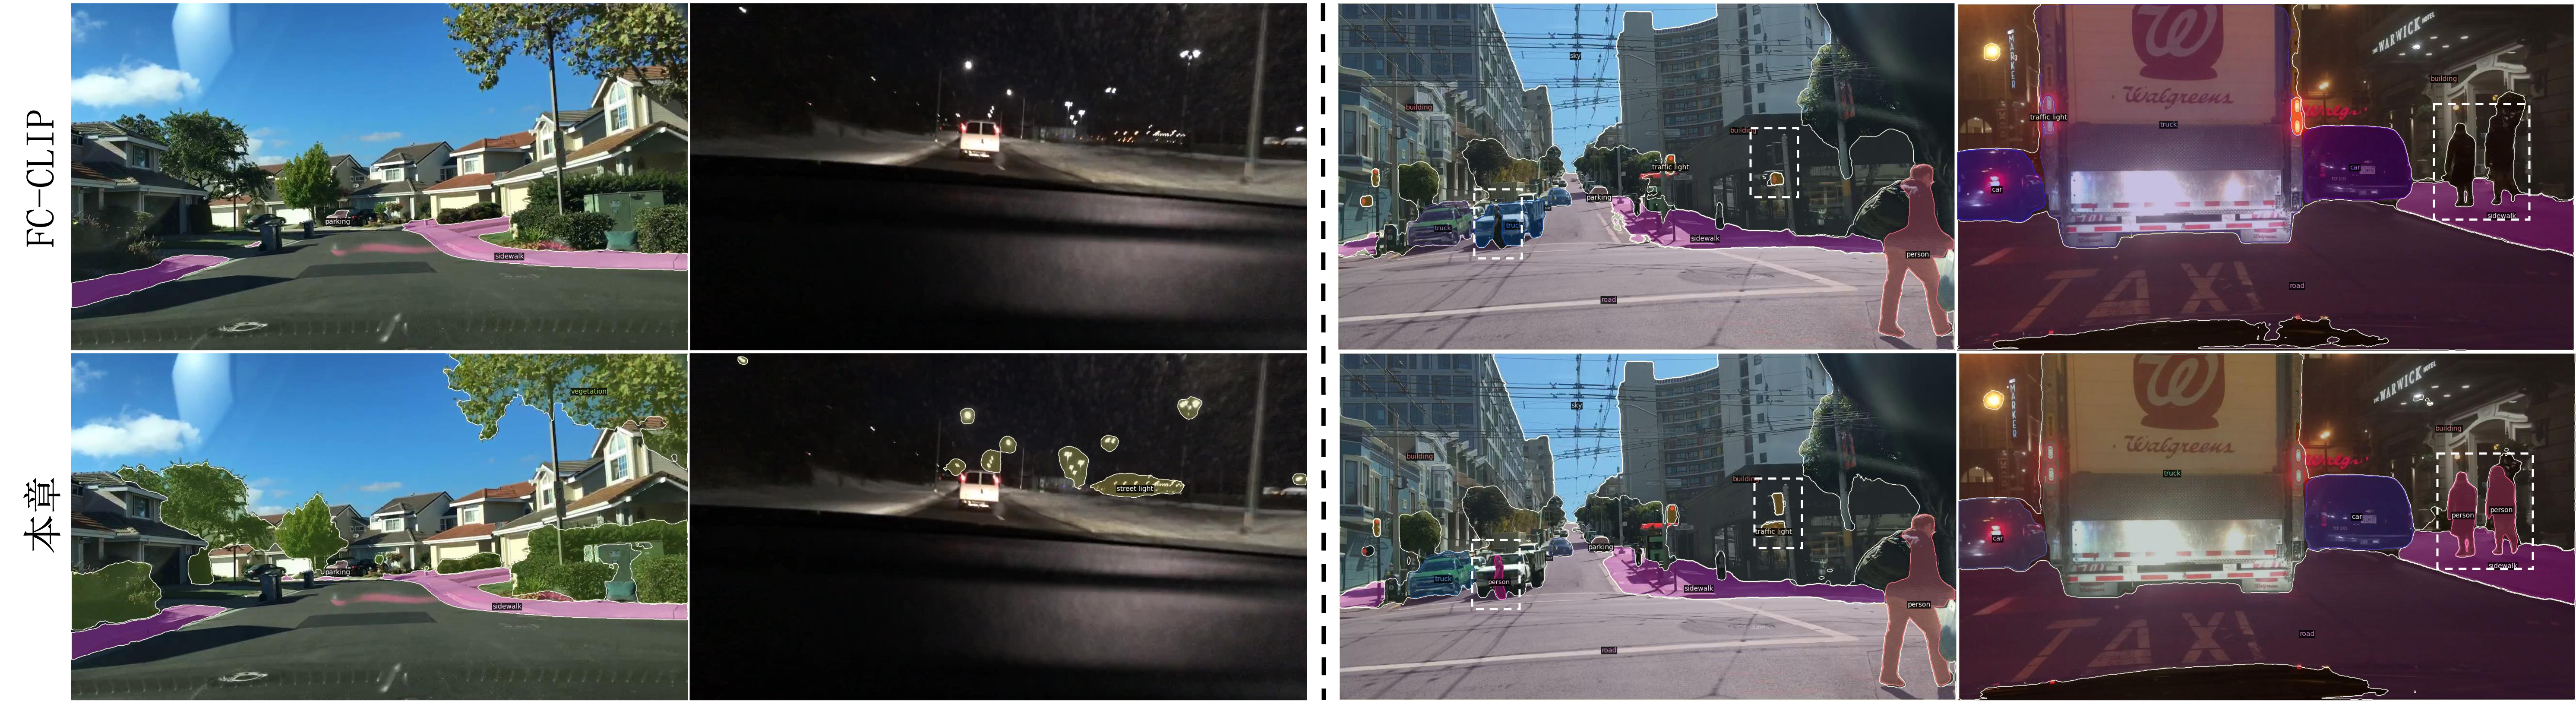
\includegraphics[width=1.\linewidth]{figures/cmpf/panop_bdd.png}
    \label{fig:cmpf_bdd}
    }
    \bicaption[fig:cmpf_city_bdd]{}{Cityscapes与BDD100K数据集上全景分割结果可视化对比}{Fig.}{Qualitative comparison of panoptic segmentation results on Cityscapes and BDD100K}
\end{figure}


表~\ref{tab:semantic_cmpf}给出了四个语义分割基准上的结果。CMPF在所有数据集上均刷新了最优性能，无论采用RN50$\times$64还是ConvNeXt-L骨干均取得明显提升；值得注意的是，CMPF仅使用COCO Panoptic的133个类别训练，而同期方法SCAN~\cite{liu2024open}使用COCO Stuff的171个类别训练且仅支持语义分割，CMPF在更少训练类别与更广任务覆盖下仍实现了更优性能，体现了该方法在数据效率与泛化能力上的双重优势。如图~\ref{fig:cmpf_pc459}与图~\ref{fig:cmpf_a847}所示，相较于MaskCLIP与FC-CLIP，CMPF在保持结构完整性与上下文一致性方面表现更优，尤其在未见类别的分割边界上展现出更强的泛化能力，可视化结果与定量数据高度一致。

\begin{table*}[!htbp]\centering
    \bicaption[tab:semantic_cmpf]{}{开放词汇语义分割结果对比}{Table}{Open-vocabulary semantic segmentation results}
    % \setlength{\tabcolsep}{2pt}
    \vspace{0.5em}\centering\wuhao
    % \resizebox{.6\textwidth}{!}{
    \begin{tabular}{llcccc}
        \toprule
        方法 & ViL Model & PC-459 & PC-59 & A-847 & A-150 \\
        \midrule
        ZegFormer~\cite{ding2022decoupling}    & ViT-B/16   & --    & --    & --    & 16.4 \\
        SimBase~\cite{xu2022simple}            & ViT-B/16   & --    & 47.7  & 7.0   & 20.5 \\
        OpenSeg~\cite{ghiasi2022scaling}       & ALIGN      & 11.2  & 45.9  & 6.8   & 24.8 \\
        OPSNet~\cite{chen2023open}             & RN50       & --    & 54.3  & --    & 25.4 \\
        \midrule
        Ovseg~\cite{liang2023open}             & ViT-L/14   & 12.4  & 55.7  & 9.0   & 29.6 \\
        MaskCLIP~\cite{ding2023open}           & ViT-L/14   & 10.0  & 45.9  & 8.2   & 23.7 \\
        MasQCLIP~\cite{MasQCLIP}         & ViT-L/14   & 18.2  & 57.8  & 10.7  & 30.4 \\
        ODISE~\cite{xu2023open}                & ViT-L/14   & 14.5  & 57.3  & 11.1  & 29.9 \\
        SCAN~\cite{liu2024open}                & ViT-L/14   & 16.7  & 59.3  & 14.0  & 33.5 \\
        \midrule
        FC-CLIP~\cite{yu2023convolutions}      & RN50$\times$64 & 15.6 & 54.8 & 10.8 & 28.7 \\
        \textbf{CMPF}                          & RN50$\times$64 & \textbf{18.7} & \textbf{57.5} & \textbf{11.8} & \textbf{30.7} \\
        \midrule
        FC-CLIP~\cite{yu2023convolutions}      & ConvNeXt-L & 17.3  & 56.6  & 14.0  & 32.8 \\
        EOV-Seg~\cite{niu2025eov}              & ConvNeXt-L & 16.8  & 56.9  & 12.8  & 32.1 \\
        \textbf{CMPF}                          & ConvNeXt-L & \textbf{19.7} & \textbf{58.4} & \textbf{14.8} & \textbf{34.4} \\
        \bottomrule
    \end{tabular}
    % }
\end{table*}


\begin{figure}[!htbp]
    \centering
    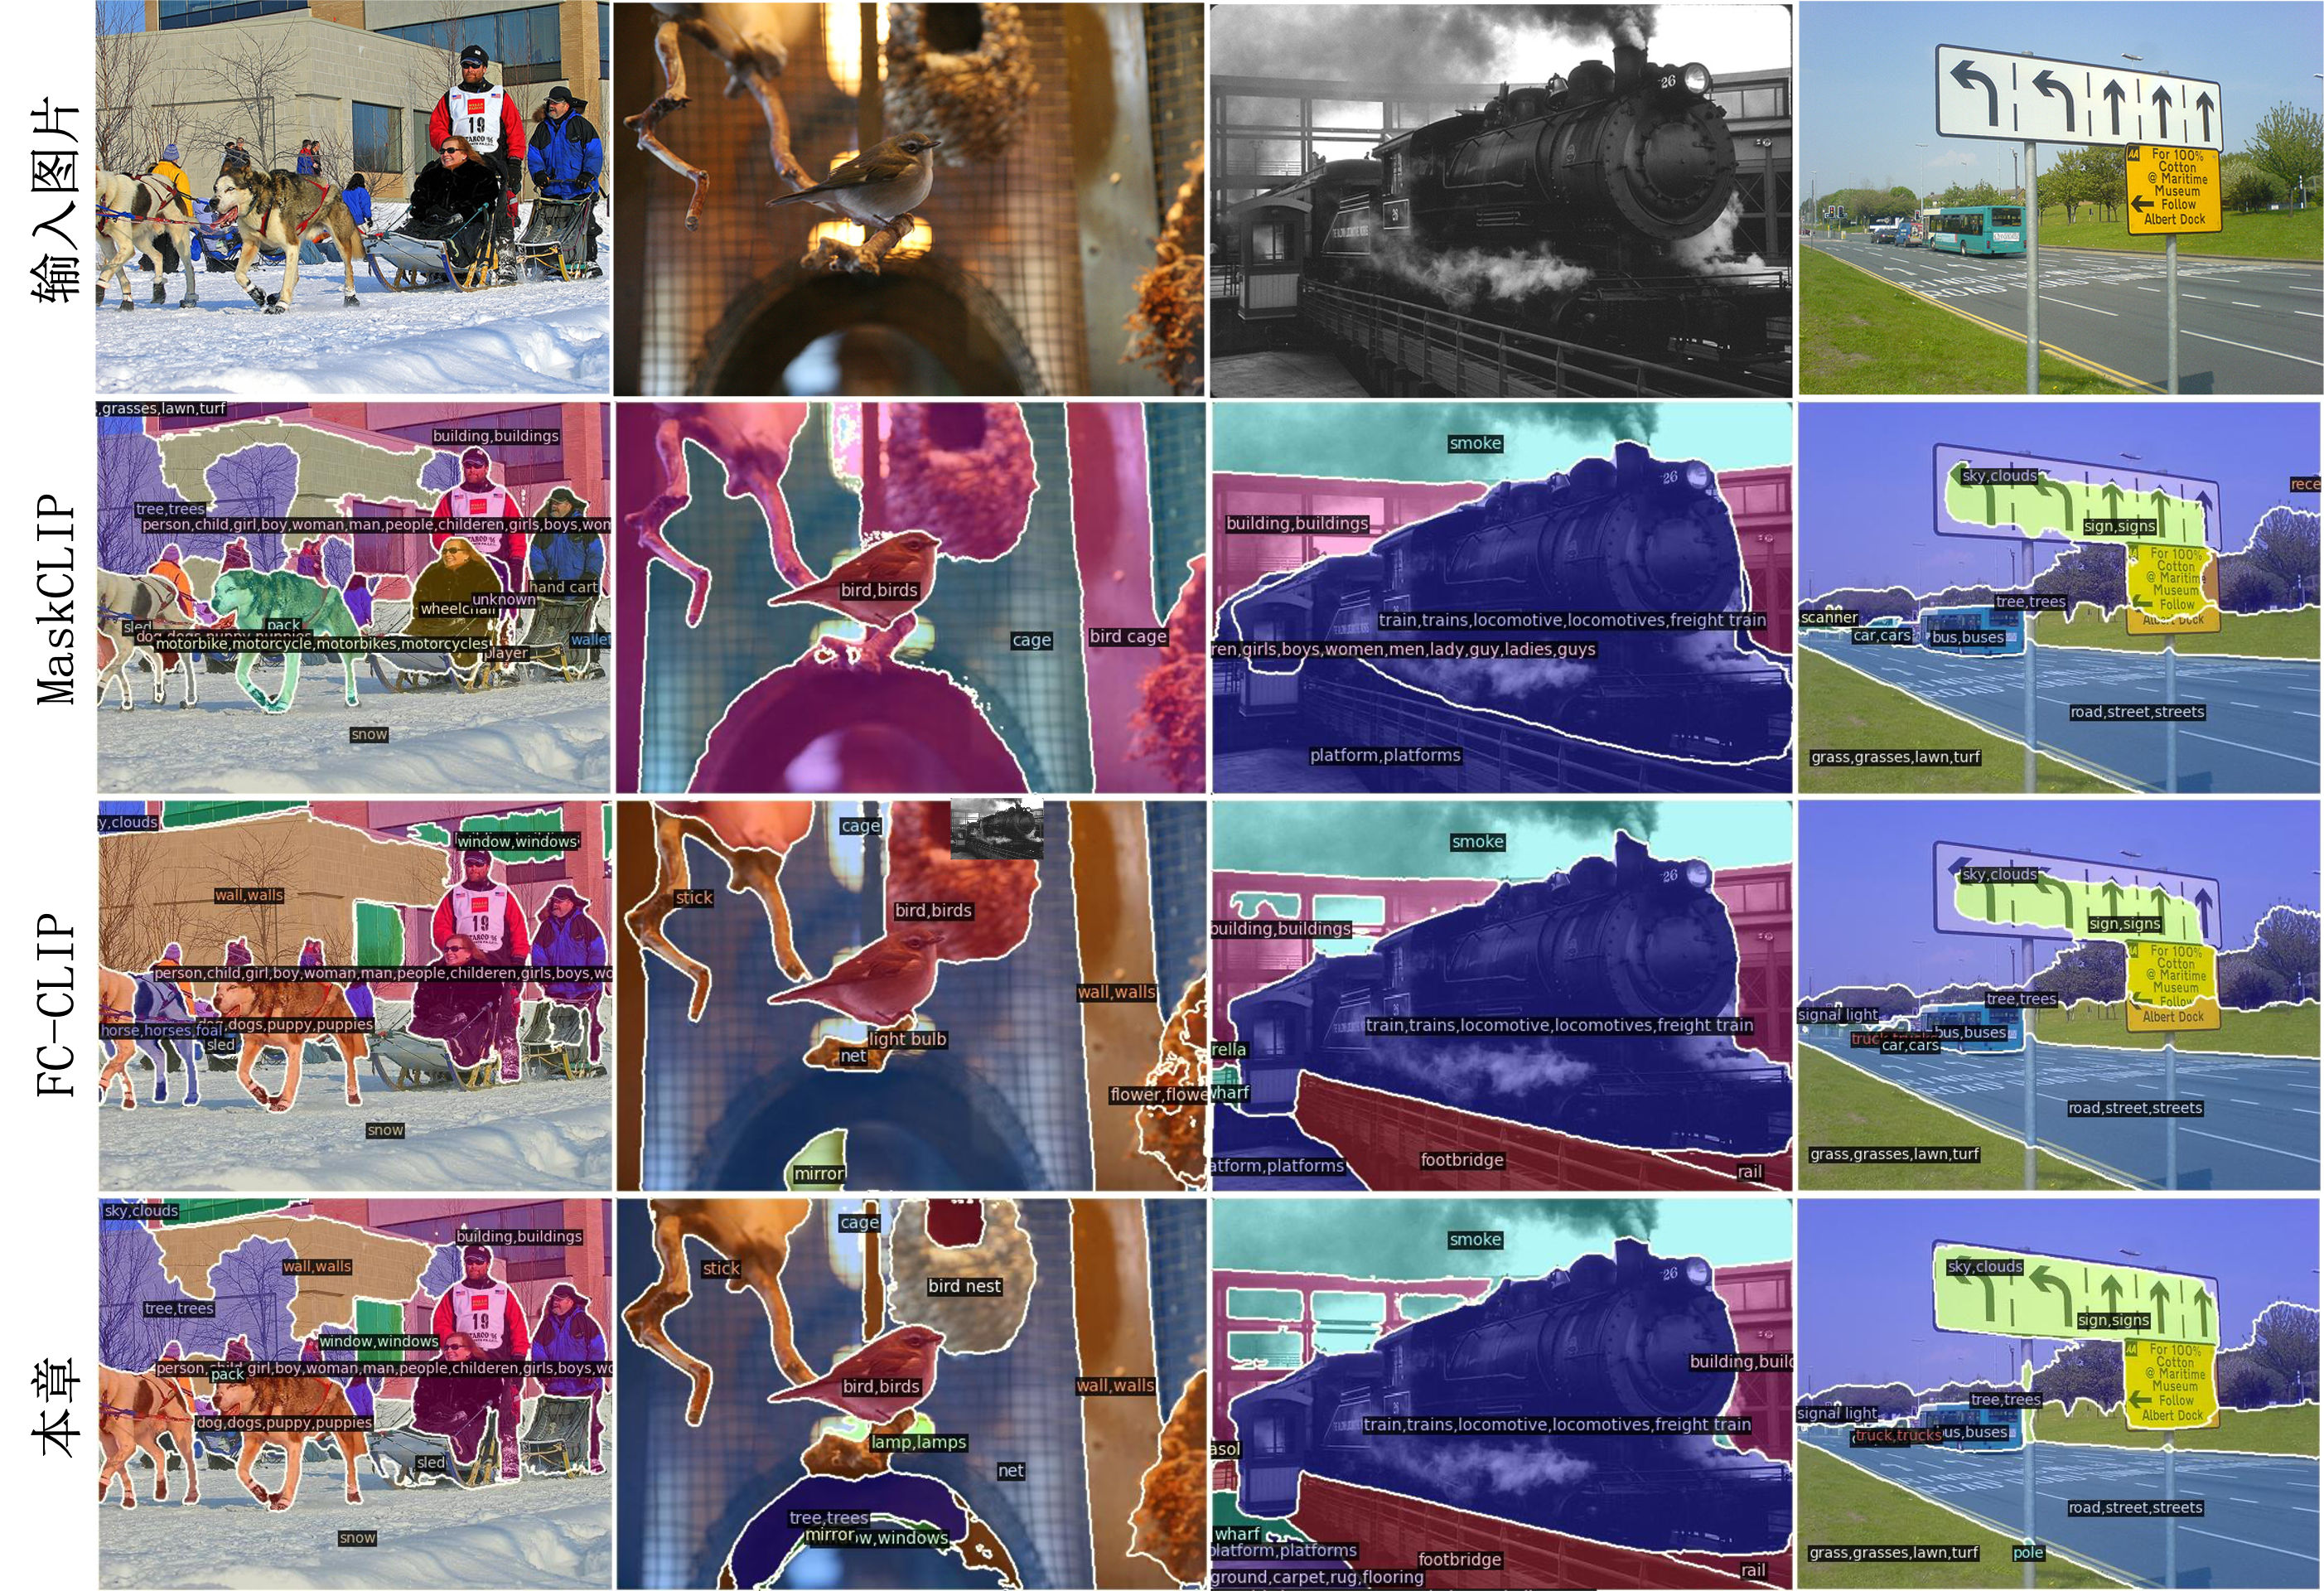
\includegraphics[width=0.95\textwidth]{figures/cmpf/sem_pc459.png}
    \bicaption[fig:cmpf_pc459]{}{PC-459数据集上语义分割结果可视化对比}{Fig.}{Qualitative comparison of semantic segmentation on PC-459}
\end{figure}

\begin{figure}[!htbp]
    \centering
    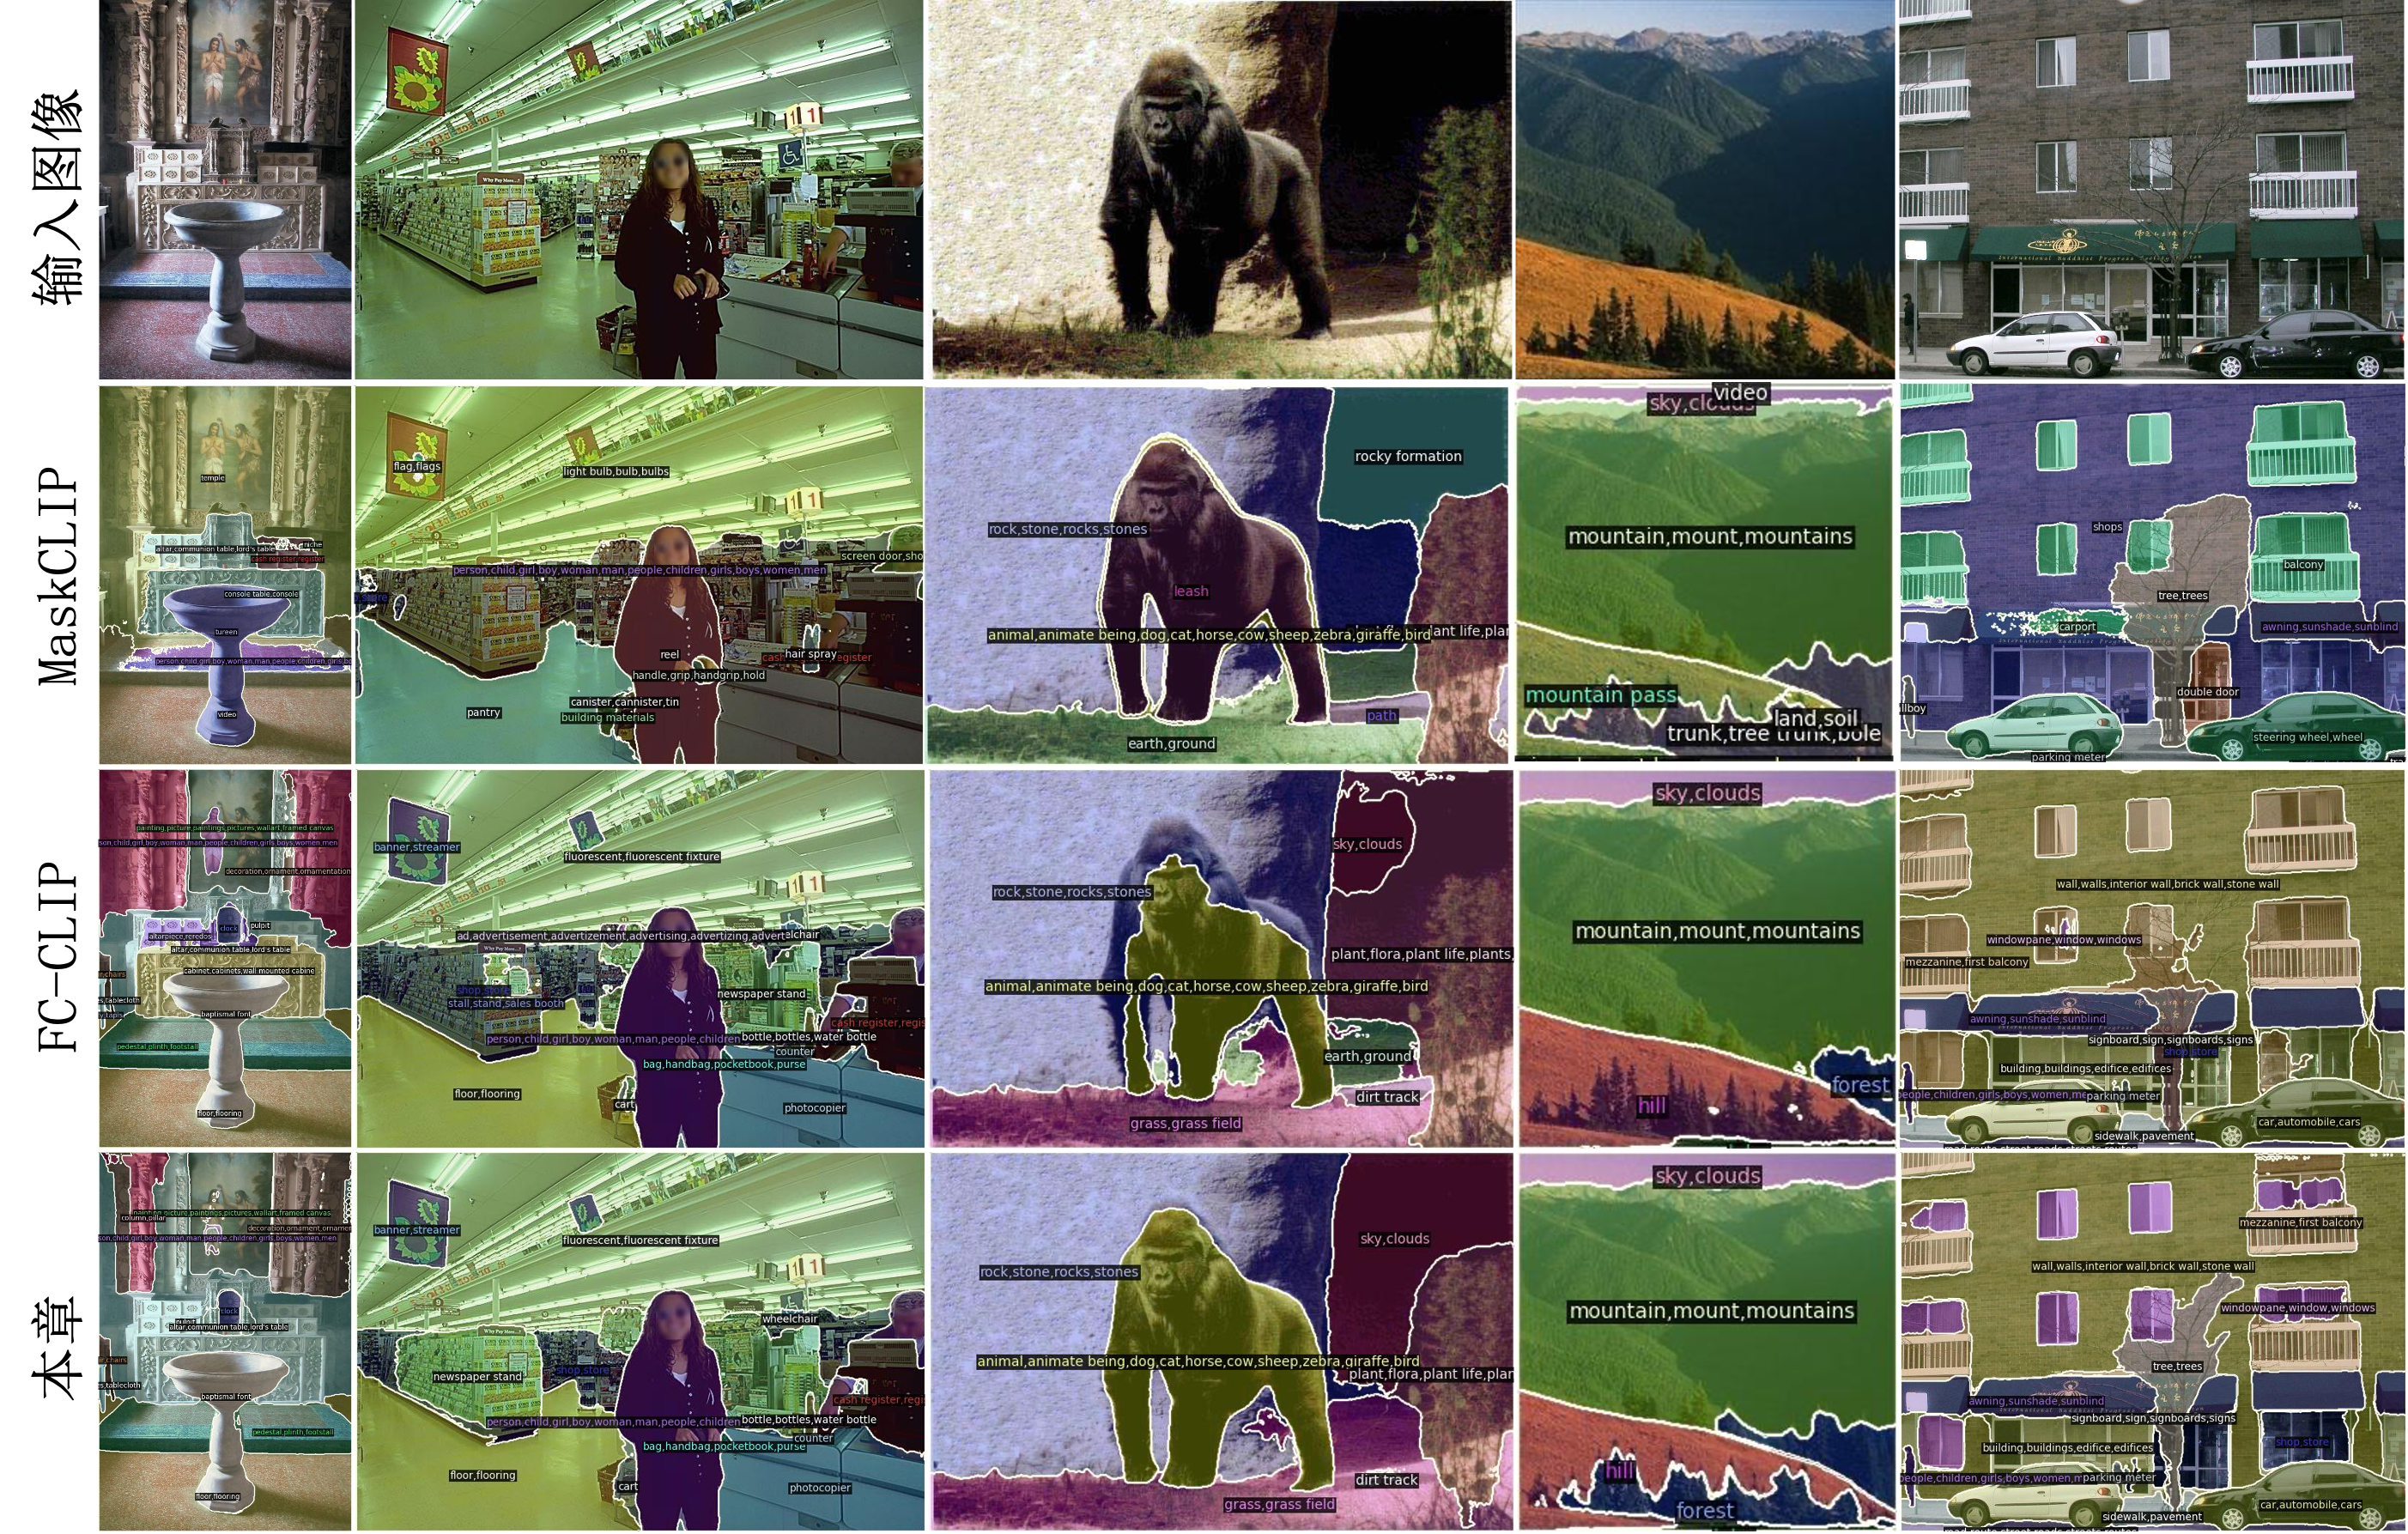
\includegraphics[width=0.95\textwidth]{figures/cmpf/sem_a847.png}
    \bicaption[fig:cmpf_a847]{}{A-847数据集上语义分割结果可视化对比}{Fig.}{Qualitative comparison of semantic segmentation on A-847}
\end{figure}

表~\ref{tab:instance_cmpf}给出了在LVIS v1.0数据集rare类别上的实例分割结果，CMPF（ConvNeXt-L）在该指标上高于RegionSpot~\cite{yang2024recognize}与Open-Vocabulary SAM~\cite{yuan2024open}等依赖额外box proposals与大规模外部数据集的方法。需要注意的是，两类对比方法的训练条件与本章方法并不相同：前者分别引入了额外的预检测器与更大规模的外部训练数据，因此该表所能支持的结论限于本章方法在更受限的训练条件下取得了当前最优的rare类别精度，而非方法本身的绝对优势；本章方法以端到端方式生成proposals，仅依赖COCO Panoptic训练，无需额外的预检测器或外部数据。


\begin{table*}[!htbp]\centering
    \bicaption[tab:instance_cmpf]{}{LVIS v1.0数据集rare类别开放词汇实例分割结果对比}{Table}{Open-vocabulary instance segmentation on LVIS rare}
    \setlength{\tabcolsep}{2pt}
    \vspace{0.5em}\centering\wuhao
    % \resizebox{.8\textwidth}{!}{%
    \begin{tabular}{lcccc}
        \toprule
        方法 & ViL Model & 训练数据 & 外部提议 & $\text{AP}_r$ \\
        \midrule
        & ViT-B/16 & O365 & GLIP-T(B) & 12.7 \\
        RegionSpot~\cite{yang2024recognize} & ViT-L/14 & O365, OI, V3D & SAM-B & 14.3 \\
        & ViT-B/16 & O365, OI, V3D & GLIP-T & 20.0 \\
        \midrule
        Open-Vocabulary SAM~\cite{yuan2024open} & RN50$\times$16 & SAM-1B+LVIS$^\ddag$ & Detic & 24.0 \\
        \midrule
        FC-CLIP~\cite{yu2023convolutions} & ConvNeXt-L & COCO Panoptic & -- & 25.0 \\
        \textbf{CMPF} & ConvNeXt-L & COCO Panoptic & -- & \textbf{25.6} \\
        \bottomrule
    \end{tabular}
    % }
\end{table*}


\begin{figure}[!htbp]
    \centering
    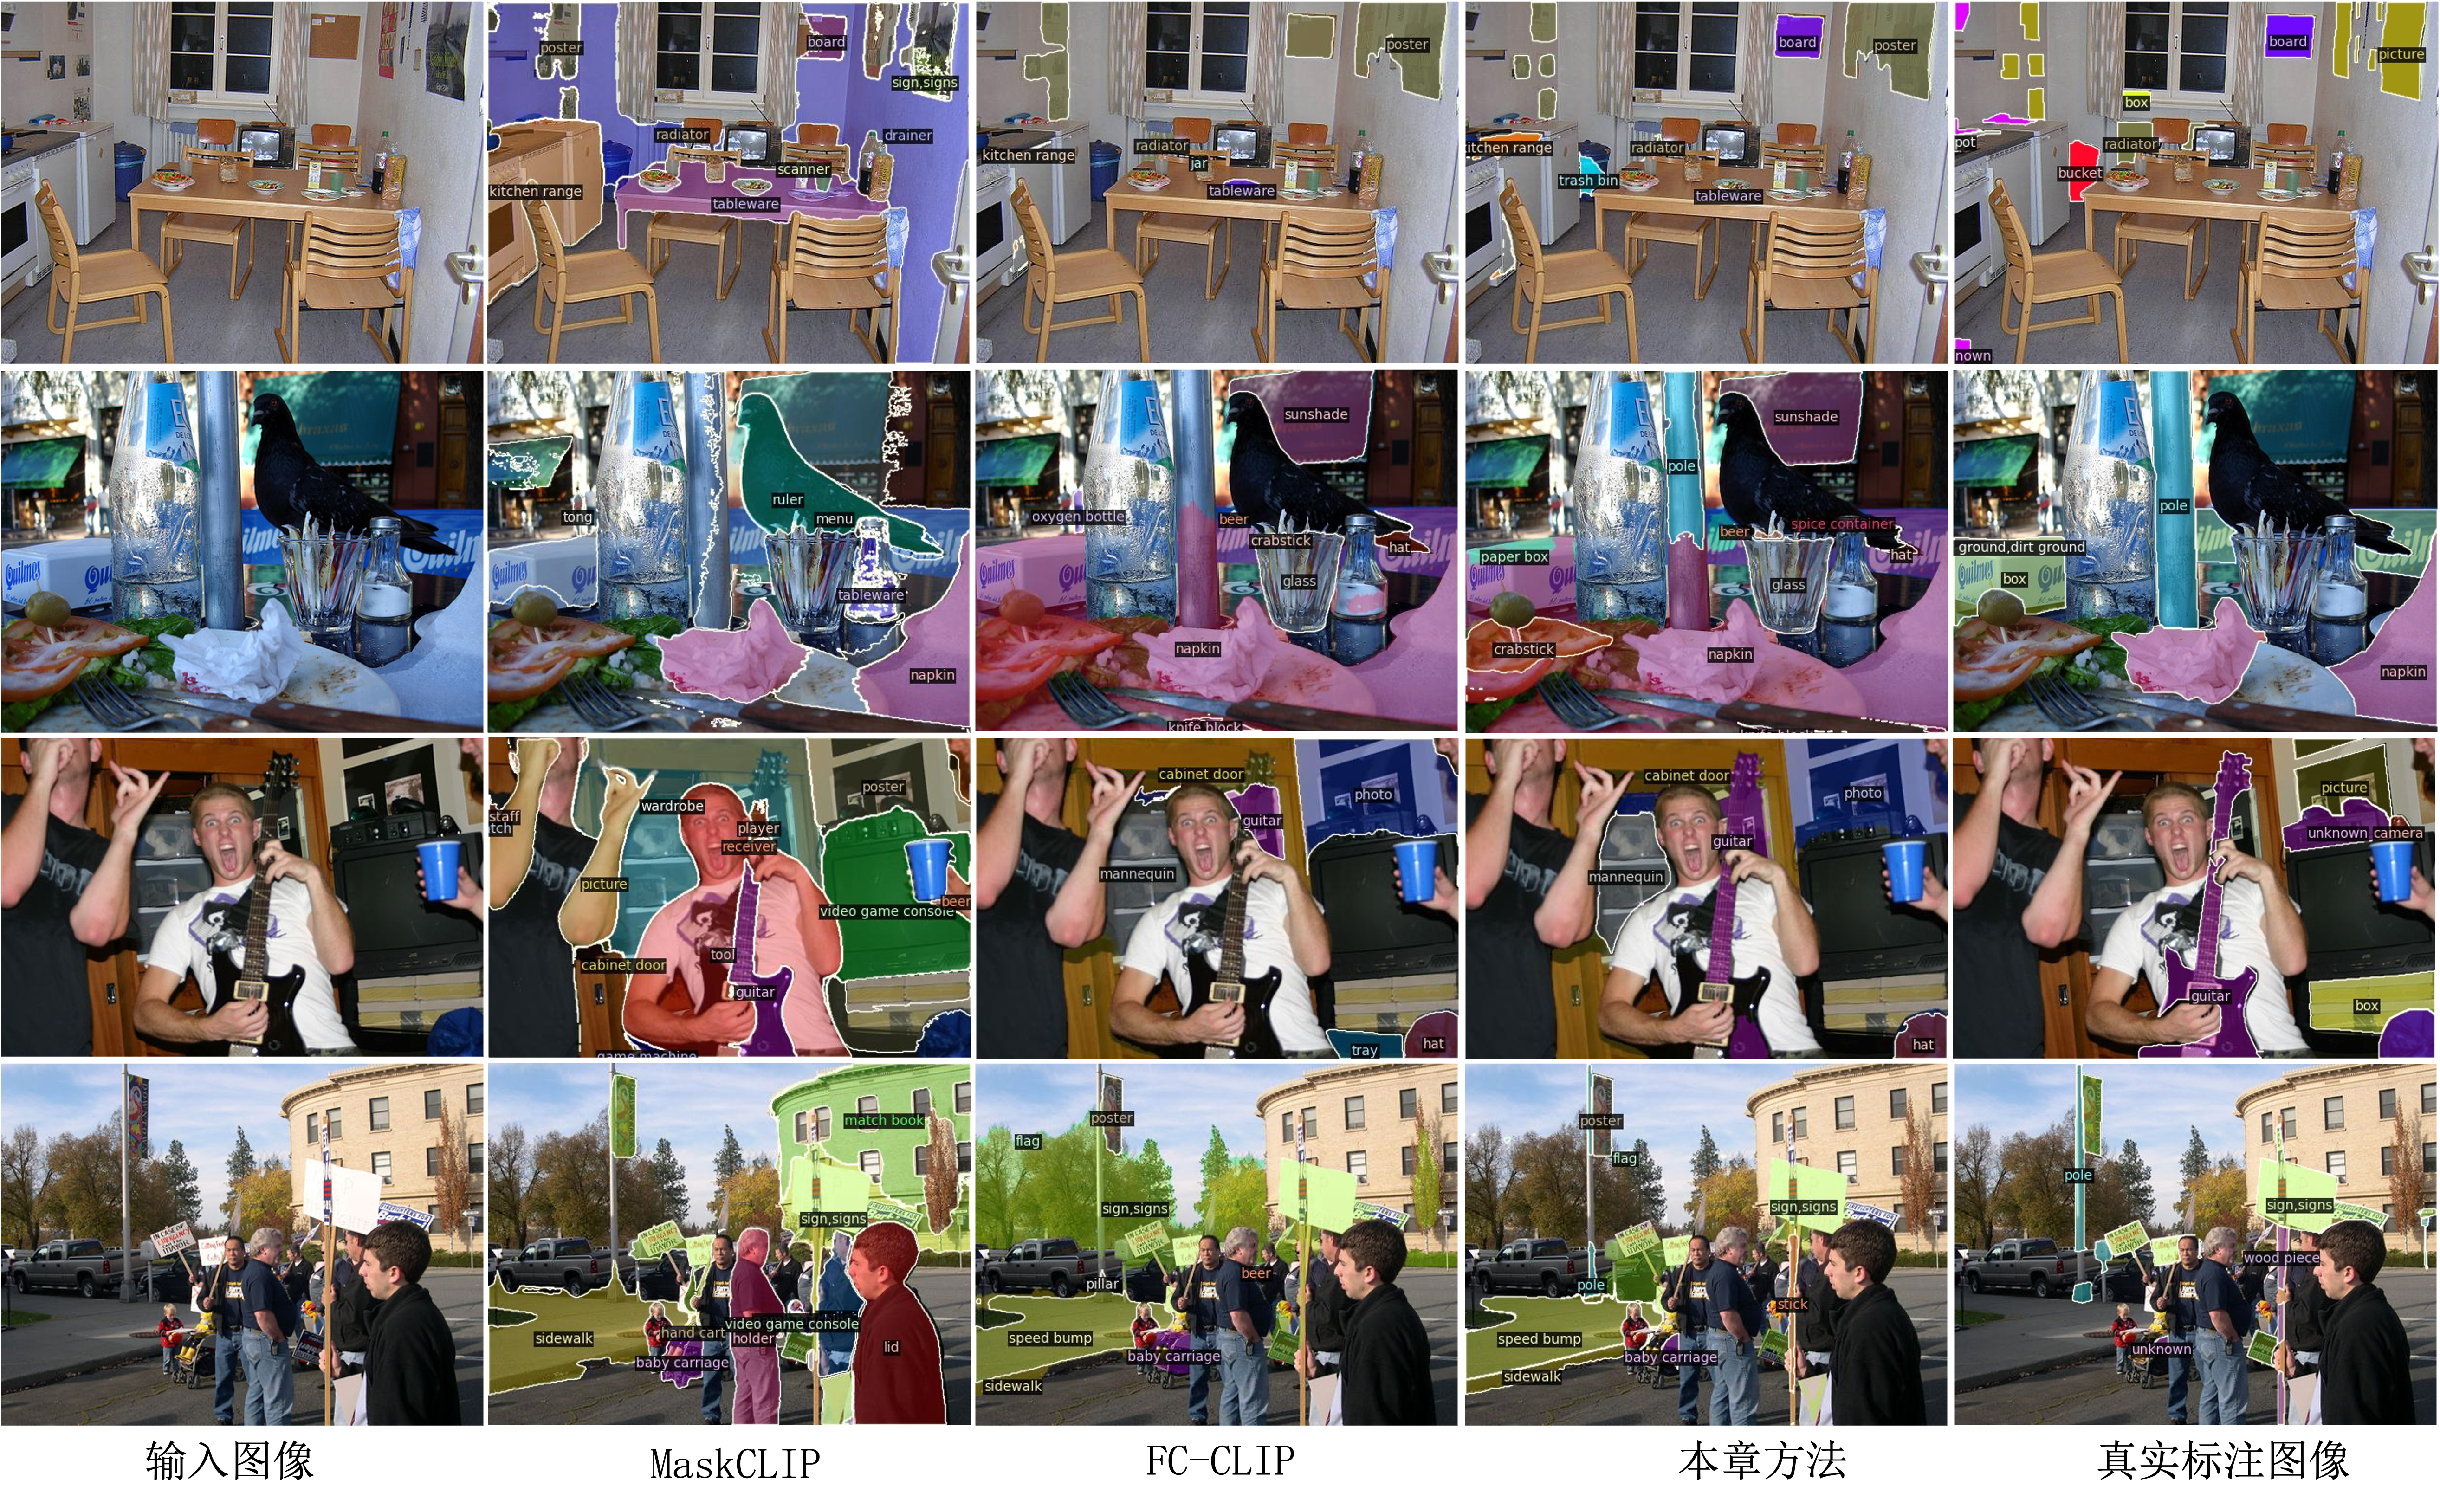
\includegraphics[width=0.95\textwidth]{figures/cmpf/Com_unseen.png}
    \bicaption[fig:cmpf_unseen]{}{PC-459数据集上未见类别零样本语义分割结果可视化}{Fig.}{Zero-shot semantic segmentation on unseen classes of PC-459}
\end{figure}

\begin{table*}[!htbp]\centering
    \bicaption[tab:unseen_cmpf]{}{开放词汇语义分割可见/未见类别mIoU对比（\%）}{Table}{mIoU on seen/unseen classes}
    \vspace{0.5em}\centering\wuhao
    \setlength{\tabcolsep}{2pt}
    \resizebox{.8\textwidth}{!}{%
    \begin{tabular}{lcccccc}
        \toprule
        \multirow{2}{*}{方法} & \multicolumn{2}{c}{PC-459} & \multicolumn{2}{c}{A-847} & \multicolumn{2}{c}{A-150} \\
        \cline{2-7}
         & $\text{mIoU}_{seen}$ & $\text{mIoU}_{unseen}$ & $\text{mIoU}_{seen}$ & $\text{mIoU}_{unseen}$ & $\text{mIoU}_{seen}$ & $\text{mIoU}_{unseen}$ \\
        \midrule
        MaskCLIP~\cite{ding2023open}  & 30.3 & 6.3 & 16.7 & 6.0 & 32.7 & 16.5 \\
        FC-CLIP~\cite{yu2023convolutions} & 46.0 & 8.7 & 34.0 & 11.3 & 47.3 & 22.0 \\
        \textbf{CMPF}                & \textbf{48.1} & \textbf{11.2} & \textbf{34.7} & \textbf{12.1} & \textbf{49.0} & \textbf{23.6} \\
        \bottomrule
    \end{tabular}}
\end{table*}


围绕未见类别这一开放词汇分割的核心场景，本节从可视化与定量两方面展开分析。PC-459数据集上“poster”、“board”、“pole”等未见类别的零样本语义分割效果优于对比方法（如图~\ref{fig:cmpf_unseen}所示），定性印证了Query Injector对掩码生成质量的提升；表~\ref{tab:unseen_cmpf}进一步从定量角度对比了CMPF在可见与未见类别上的分割表现，未见类别上取得提升的同时，可见类别上也保持竞争力，表明SAM空间先验的融合不仅强化了开放词汇泛化能力，也未损害对训练类别的判别精度。

表~\ref{tab:recall_cmpf}从掩码质量角度报告了不同IoU阈值（0.5/0.75/0.9）下的召回率，CMPF在所有阈值上均显著优于FC-CLIP在未见类别上的掩码提议，验证了Query Injector对掩码生成质量的系统性提升。

\begin{table*}[!htbp]
    \bicaption[tab:recall_cmpf]{}{开放词汇语义分割掩码召回率}{Table}{Open-vocabulary semantic mask recall }
    \vspace{0.5em}\centering\wuhao
    \setlength{\tabcolsep}{1pt}
    \resizebox{\textwidth}{!}{
    \begin{tabular}{lccccccccc}
        \toprule
        \multirow{2}{*}{方法} & \multicolumn{3}{c}{PC-459 (S/U)} & \multicolumn{3}{c}{A-847 (S/U)} & \multicolumn{3}{c}{A-150 (S/U)} \\
        \cline{2-10}
         & 0.5 & 0.75 & 0.9 & 0.5 & 0.75 & 0.9 & 0.5 & 0.75 & 0.9 \\
        \midrule
        FC-CLIP & 91.4/77.7 & 73.6/56.2 & 43.9/28.4 & \textbf{84.6}/66.6 & \textbf{60.0}/41.3 & \textbf{27.6}/14.3 & 83.7/72.0 & 58.9/45.5 & \textbf{27.7}/17.4 \\
        \textbf{CMPF} & \textbf{92.6/81.0} & \textbf{76.0/59.9} & \textbf{47.0/31.4} & 78.9/\textbf{82.9} & 52.3/\textbf{59.4} & 23.6/\textbf{24.6} & \textbf{84.7}/\textbf{73.2} & \textbf{60.1}/\textbf{47.2} & 27.6/\textbf{18.0} \\
        \bottomrule
    \end{tabular}}
\end{table*}


\FloatBarrier
\noindent\textbf{(3)消融实验分析}

表~\ref{tab:ablation_cmpf}给出了CMPF三个核心组件的消融结果。单独使用SAM的proposals时，三个数据集上的性能说明SAM具有基础泛化能力但缺乏语义指导。在统一框架下逐步加入三个模块，指标持续提升：Query Injector引入细粒度空间查询后性能大幅改善，Feature Injector进一步精炼了语义—空间特征融合，OpenSeg Ensemble在推理阶段提供了互补增益。值得注意的是，仅依靠OpenSeg Ensemble的提升有限，说明SAM空间信息的深度融合——即两个Injector——是性能提升的主要驱动力。

\begin{table}[!htbp]\centering
    \bicaption[tab:ablation_cmpf]{}{CMPF各模块消融结果}{Table}{Ablation of CMPF components}
    \vspace{0.5em}\centering\wuhao
    \setlength{\tabcolsep}{2pt}
    \begin{tabular}{cccccccc}
        \toprule
        &\multirow{2}{*}{Query Injector} & \multirow{2}{*}{Feature Injector} & \multirow{2}{*}{OpenSeg Ensemble} & \multicolumn{3}{c}{Semantic} & Panoptic \\
        \cline{5-8}
        & &       &       & PC-459 & A-847 & A-150 & A-150 (PQ) \\
        \midrule
        Model 1&$\times$ & $\times$ & $\times$ & 17.3 & 14.0 & 32.8 & 25.1 \\
        Model 2&$\times$ & $\times$ & \checkmark & 17.6 & 14.5 & 33.5 & -- \\
        Model 3&$\checkmark$ & $\times$ & $\times$ & 18.1 & 14.2 & 33.6 & 25.7 \\
        Model 4&$\checkmark$ & $\checkmark$ & $\times$ & 18.5 & 14.4 & 33.8 & 25.9 \\
        CMPF   & $\checkmark$& $\checkmark$ & $\checkmark$ & \textbf{19.7} & \textbf{14.8} & \textbf{34.4} & -- \\
        \bottomrule
    \end{tabular}
\end{table}


表~\ref{tab:layer_cmpf}探究了Query Injector在不同解码器层插入对性能的影响。CLIP的$1/8$分辨率特征对应解码器层$3,6,9$，实验表明在该分辨率注入SAM query能获得最佳效果。这说明Query Injector应在解码器的中后段介入，使新引入的空间查询在后续层中与CLIP特征充分交互，从而实现多轮语义精炼。

\begin{table*}[!htbp] \centering
    \bicaption[tab:layer_cmpf]{}{Query Injector插入层数对性能的影响}{Table}{Impact of injection layer in decoder}
    \vspace{0.5em}\centering\wuhao
    \setlength{\tabcolsep}{10pt}
    \resizebox{.9\textwidth}{!}{%
        \begin{tabular}{cccccccc}
            \toprule
            \multirow{2}{*}{特征尺度（插入层）} & \multirow{2}{*}{Layers} & \multicolumn{3}{c}{COCO (Seen)} & \multicolumn{3}{c}{Cityscapes} \\
            \cline{3-8}
             &  & PQ & AP & mIoU & PQ & AP & mIoU \\
            \midrule
            1/32 (1, 4, 7) & 1, 4, 7 & 52.6 & 42.7 & 62.6 & \textbf{40.4} & 20.8 & 53.0 \\
            1/16 (2, 5, 8) & 2, 5, 8 & 52.5 & 42.5 & 62.4 & 40.1 & 20.7 & 53.3 \\
            1/8 (3, 6, 9) & 3, 6, 9 & \textbf{52.7} & \textbf{42.8} & \textbf{62.7} & 40.0 & \textbf{21.6} & \textbf{54.0} \\
            \bottomrule
        \end{tabular} }%
\end{table*}


表~\ref{tab:sam_cmpf} 对比了不同规模 SAM 骨干对 CMPF 性能的影响，该结果同时是训练阶段选型依据的来源。ViT-B 规模在所有数据集上均取得最佳或近最佳性能：其 Cityscapes 全景分割 PQ 达到 45.8\%，高于 ViT-L 与 ViT-H 的 44.2\%；语义分割上 PC-459 取得 18.5\%，亦优于其他三种配置。这一结果与前述设计依据相互印证——训练阶段需要的是实例可分性而非边界精细度，ViT-T 提供的边界较粗、实例连通性不足，ViT-L/ViT-H 虽然单点精度更高，但实例连通性有所下降，对全景分割的整体质量构成不利影响。ViT-B 规模因此在分割精度与实例连通性之间取得平衡，被确定为训练阶段的编码器配置。

\begin{table}[!htbp]\centering
    \bicaption[tab:sam_cmpf]{}{不同SAM骨干规模对CMPF性能的影响}{Table}{Effect of SAM backbone size}
    \vspace{0.5em}\centering\wuhao
    % \setlength{\tabcolsep}{2pt}
    % \resizebox{.5\textwidth}{!}{
    \begin{tabular}{lcccccc}
        \toprule
        \multirow{2}{*}{SAM} & \multicolumn{3}{c}{Cityscapes} & \multicolumn{3}{c}{Semantic} \\
        \cline{2-7}
         & PQ & AP & mIoU & PC-459 & A-847 & PC-59 \\
        \midrule
        ViT-T & 43.0 & 25.9 & 55.0 & 17.6 & 14.0 & 56.8 \\
        \textbf{ViT-B} & \textbf{45.8} & \textbf{28.4} & \textbf{56.8} & \textbf{18.5} & \textbf{14.4} & \textbf{58.1} \\
        ViT-L & 44.2 & 27.1 & 56.2 & 17.4 & 14.2 & 56.7 \\
        ViT-H & 44.2 & 28.0 & 56.2 & 17.3 & 13.9 & 56.6 \\
        \bottomrule
\end{tabular}
% }
\end{table}


\begin{figure}[!htbp]
    \centering
    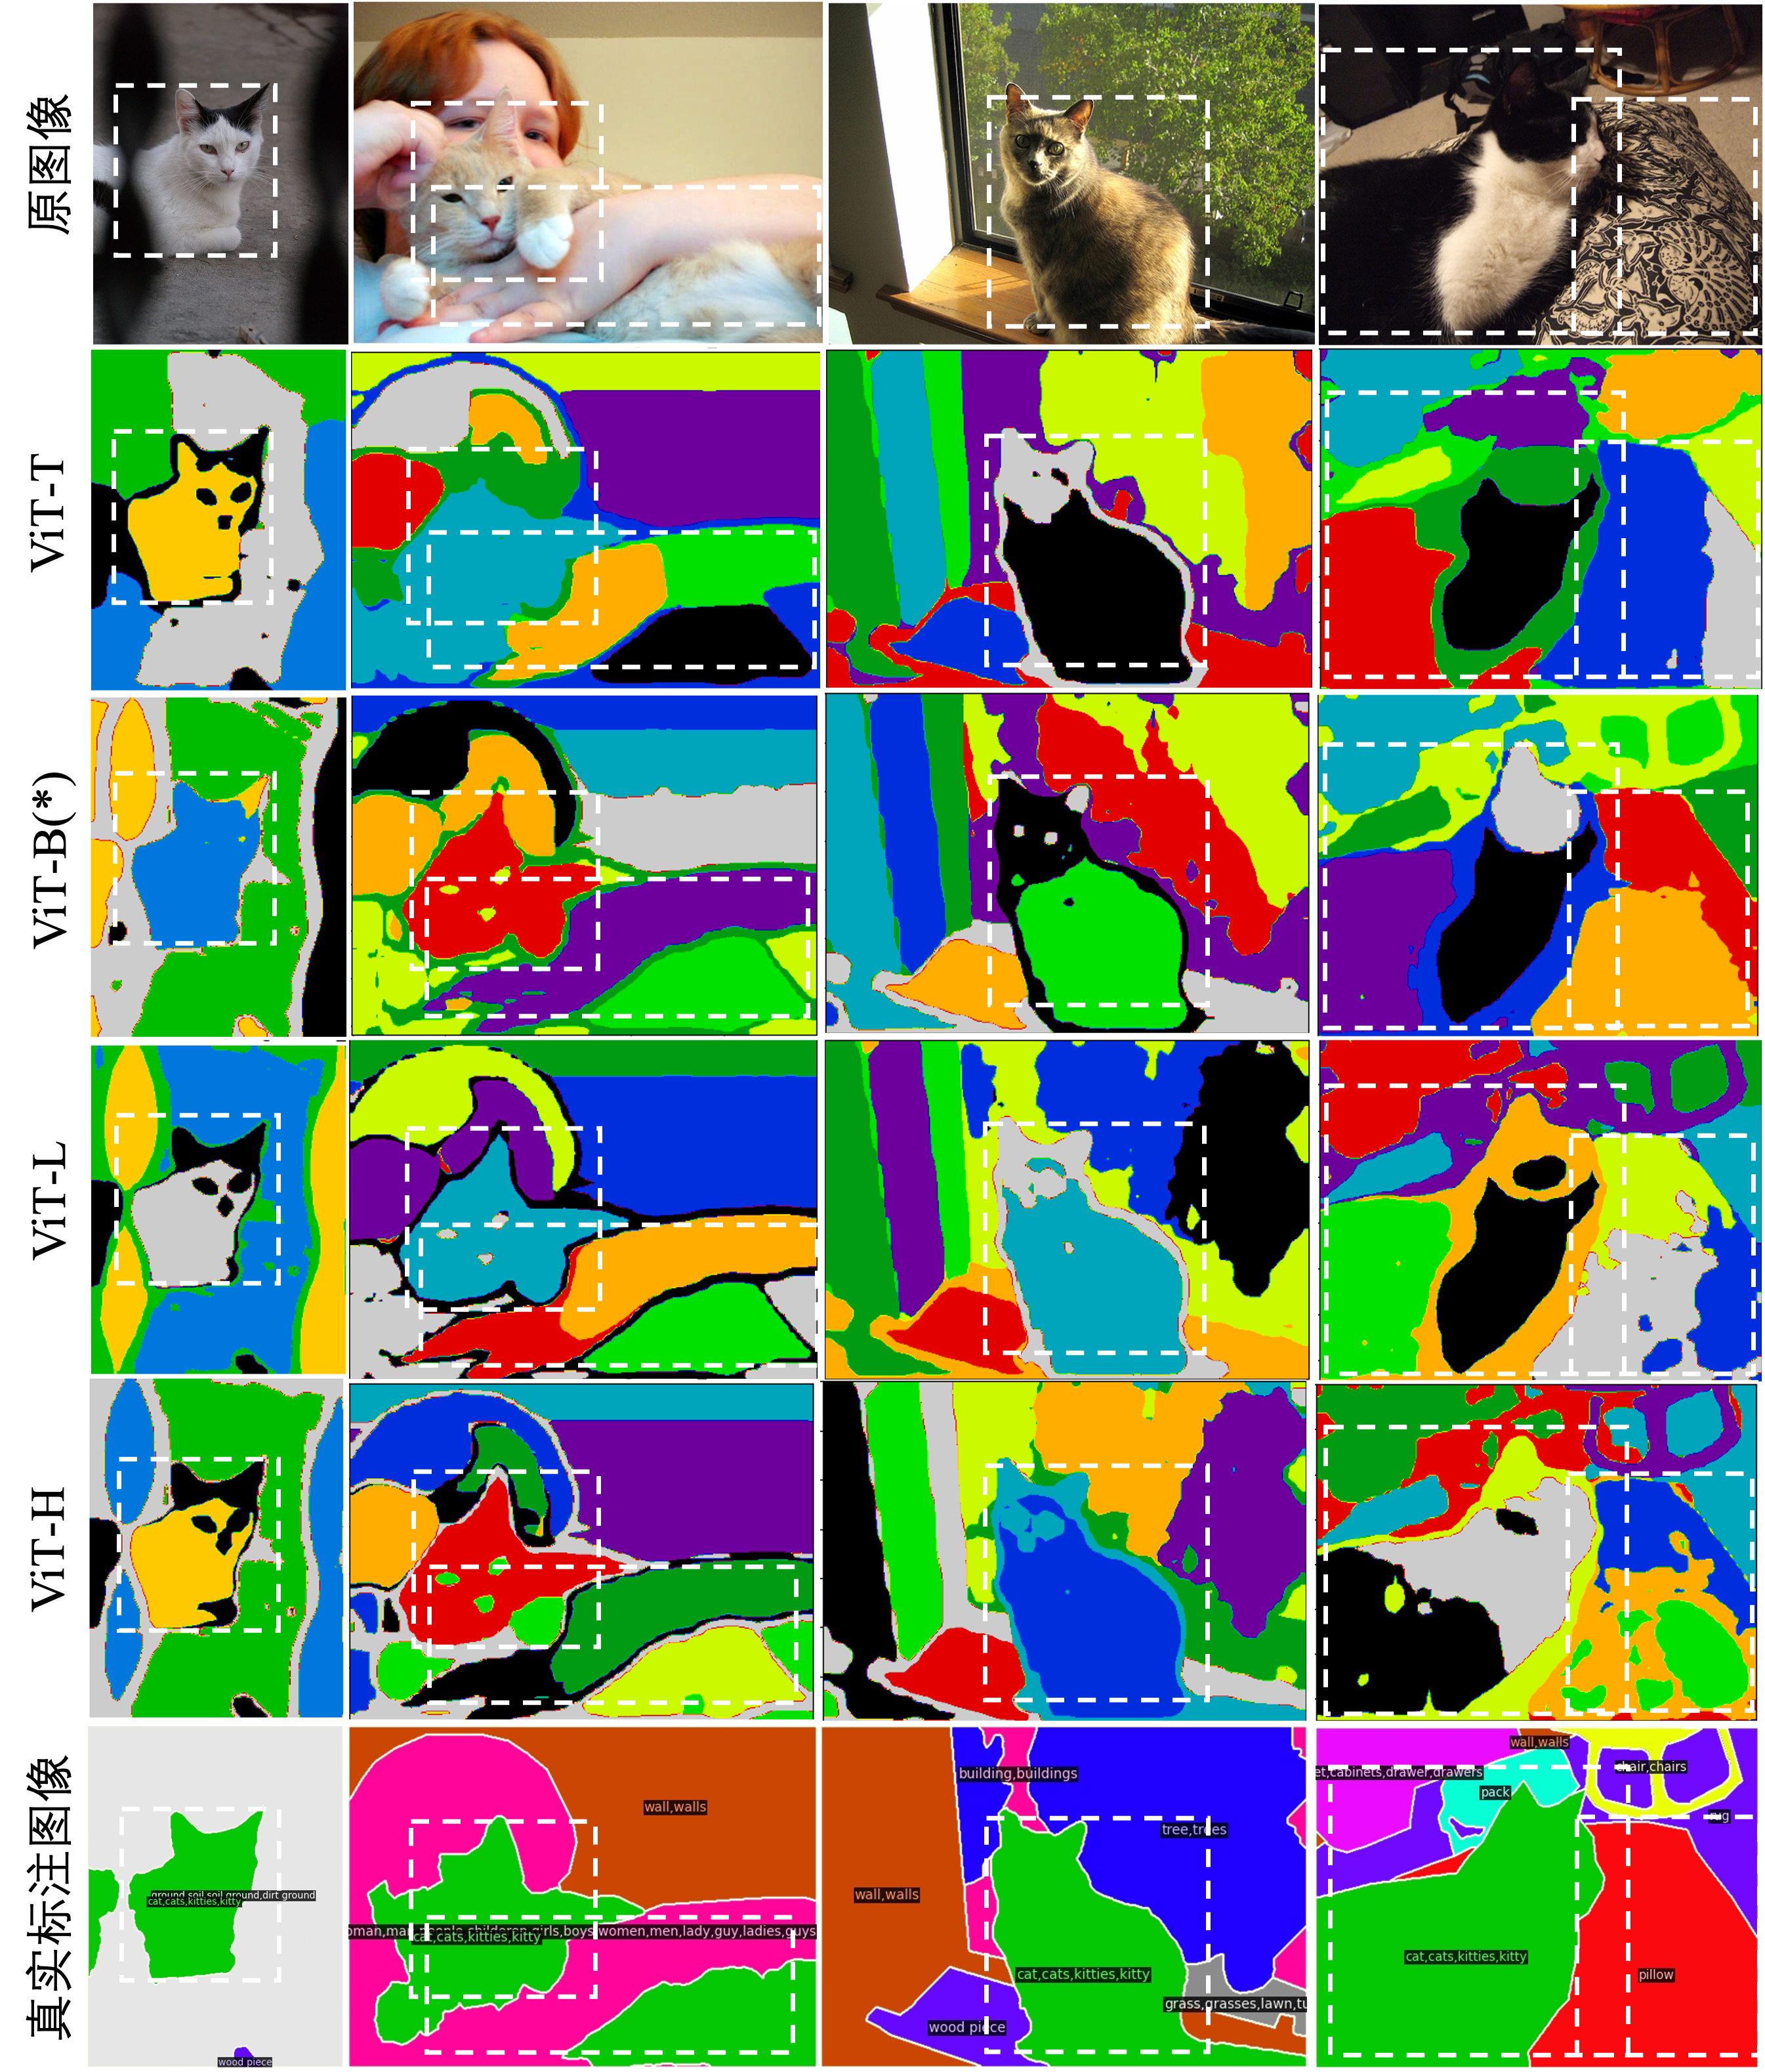
\includegraphics[width=0.65\textwidth]{figures/cmpf/sam_variants.png}
    \bicaption[fig:sam_variants]{}{不同SAM编码器在PC-459数据集上的特征嵌入k-means聚类可视化}{Fig.}{K-means clustering visualization of SAM encoder feature embeddings on PC-459}
\end{figure}

图~\ref{fig:sam_variants}给出了不同SAM图像编码器在PC-459数据集上的特征嵌入k-means聚类可视化。ViT-B编码器展现出更优的实例级连通性理解，在精确分割与实例连通之间取得了良好的平衡，与定量结果一致。



图~\ref{fig:sam_atten}给出了SAM在box提示下生成的分割掩码概率分布热力图。结果表明，SAM在给定box提示时能够对目标物体产生高注意力并有效抑制边缘区域，展现出稳健的零样本泛化能力，定性地验证了其在边界描绘方面的优势。

\begin{figure}[!htbp]
    \centering
    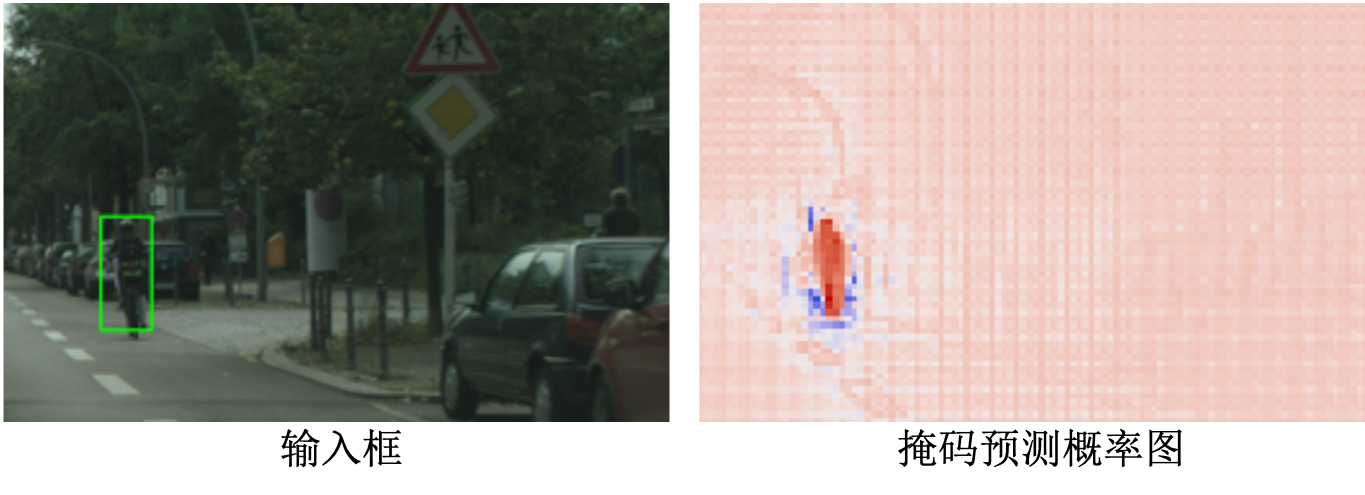
\includegraphics[width=0.75\textwidth]{figures/cmpf/sam_atten.png}
    \bicaption[fig:sam_atten]{}{SAM在box提示下生成的分割掩码概率分布热力图}{Fig.}{Probability distribution heatmap of SAM-generated segmentation masks under box prompting}
\end{figure}

图~\ref{fig:abl_atten}给出了不同消融设置下的实例级注意力图对比。单独使用CLIP时，模型对未见类别的激活区域有限；引入Query Injector后，模型能够激活先前未识别的物体区域，尤其对未见类别效果显著；Feature Injector则进一步精炼了注意力的空间分布，使激活模式更加完整和一致。两个Injector在增强物体定位与空间一致性方面发挥着互补的协同作用。

\begin{figure}[!htbp]
    \centering
    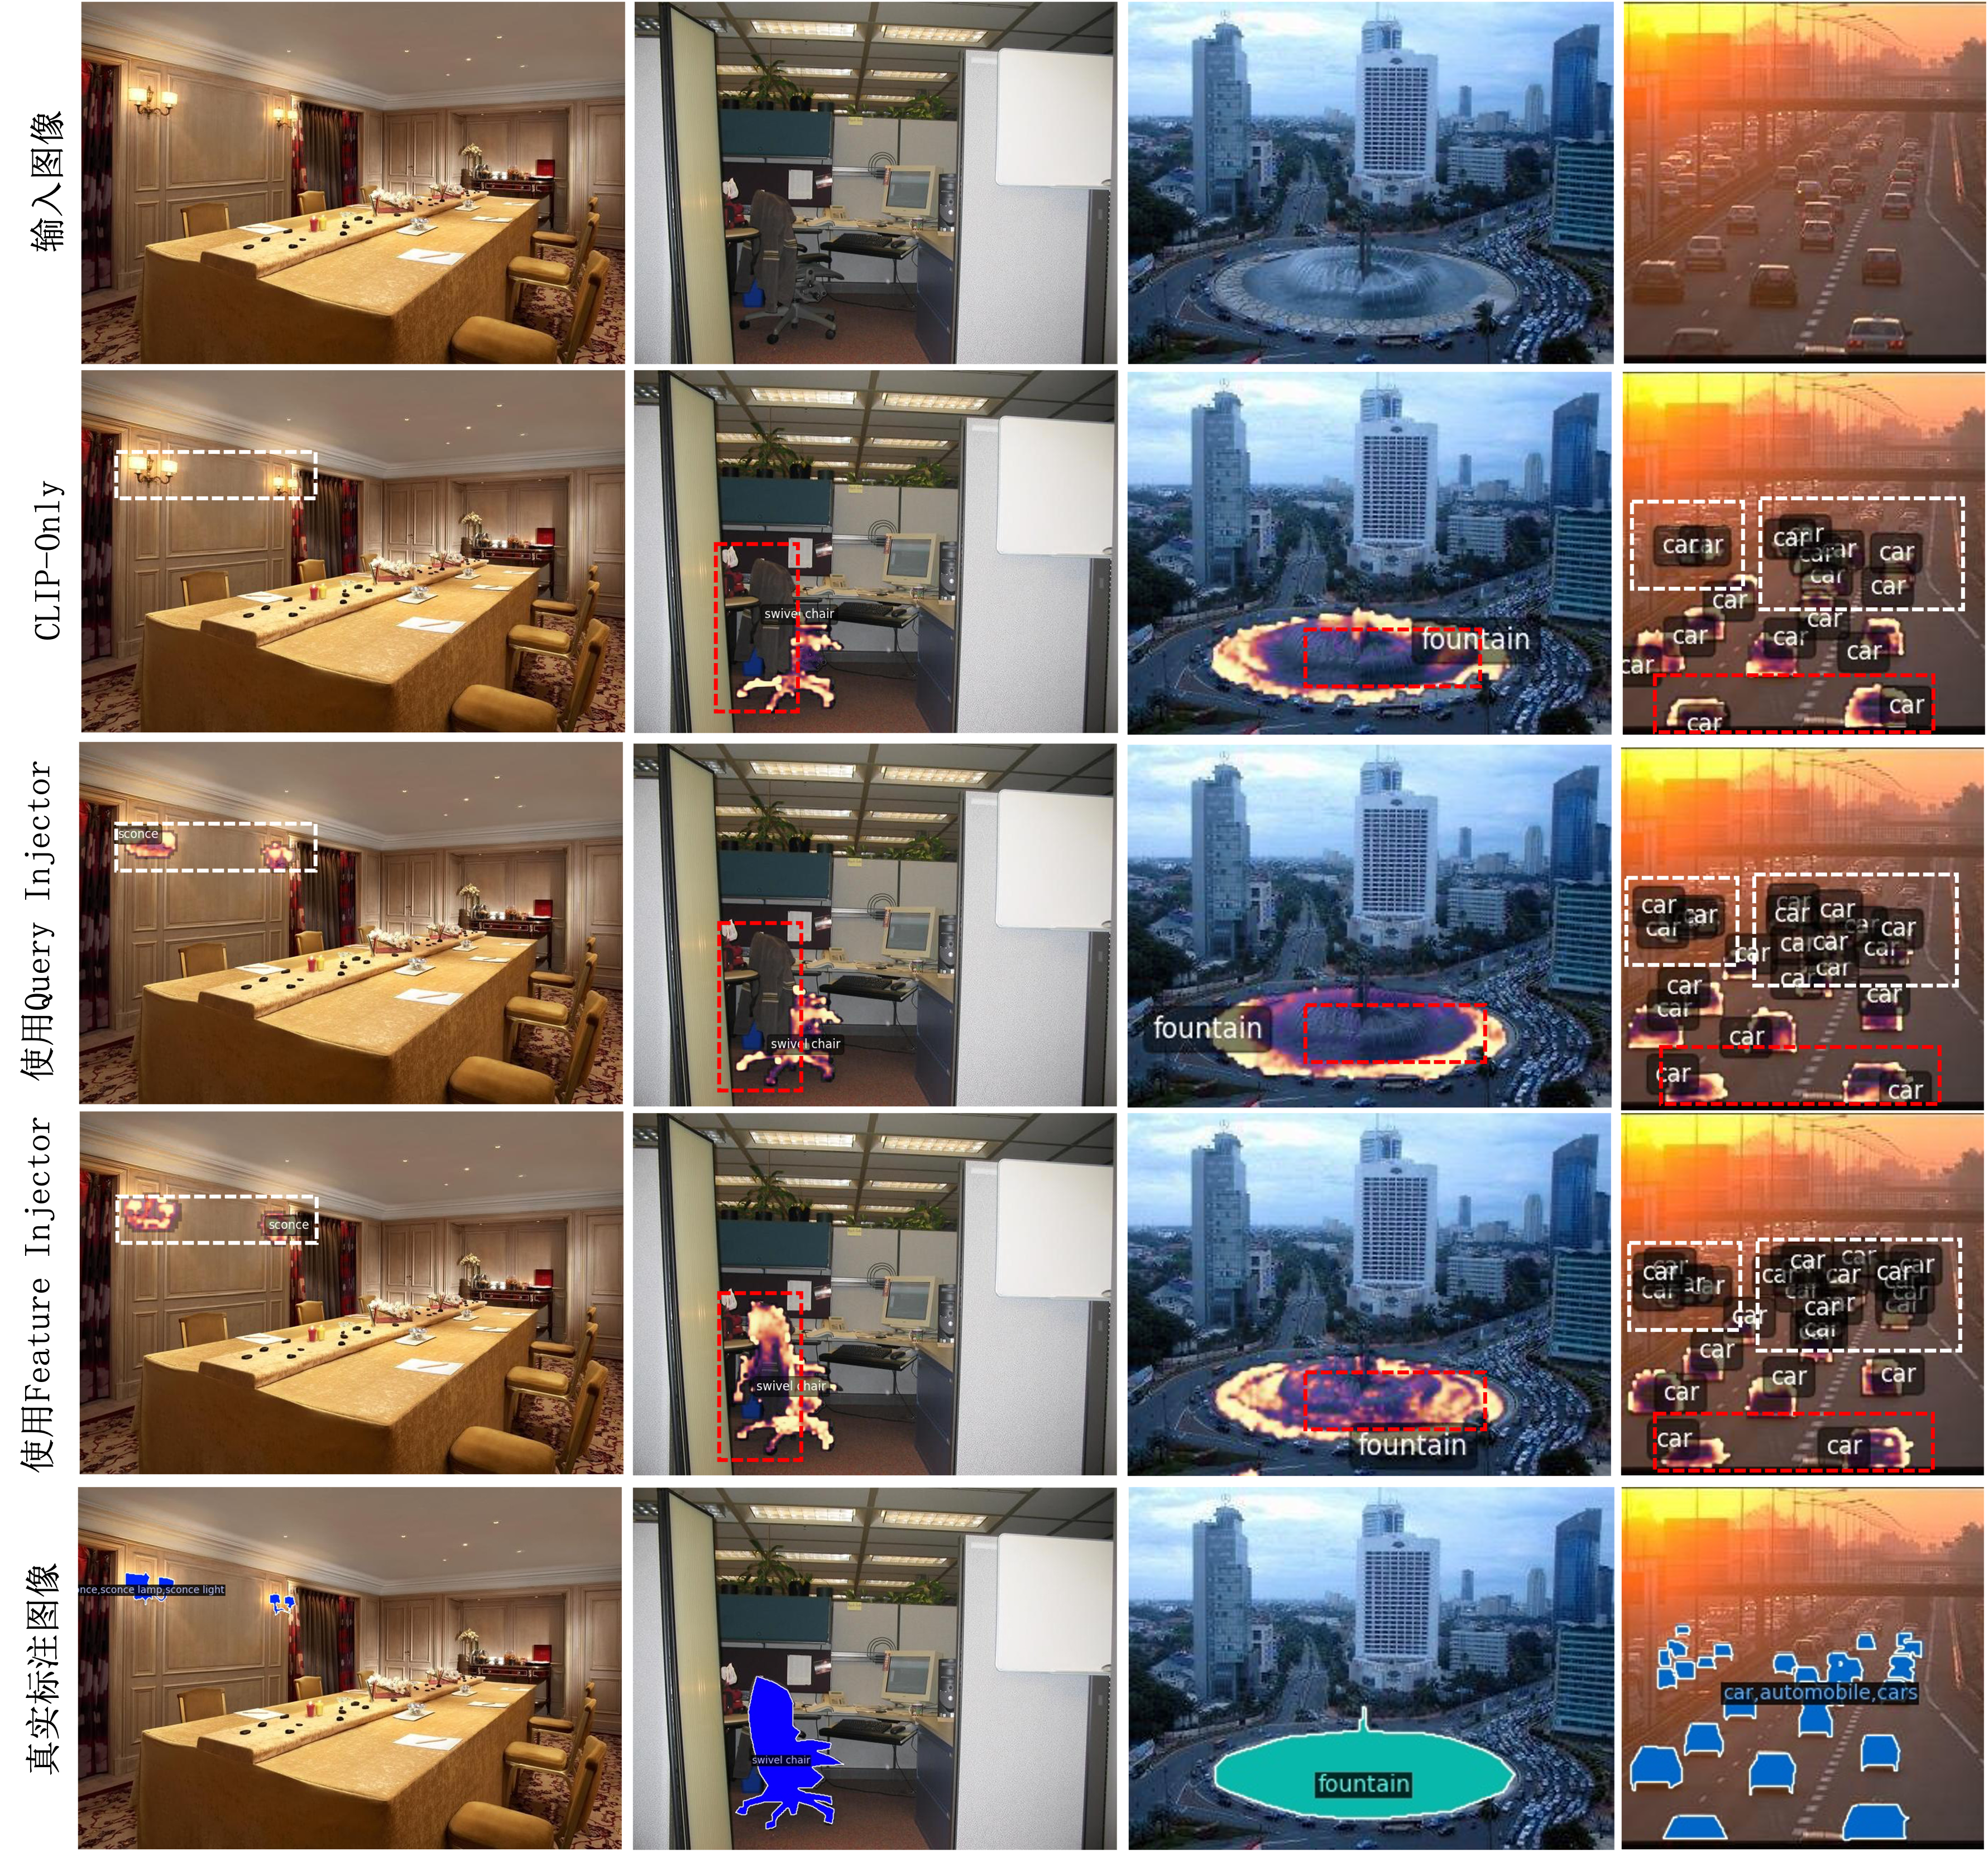
\includegraphics[width=0.95\textwidth]{figures/cmpf/abl_atten2.png}
    \bicaption[fig:abl_atten]{}{ADE20K数据集上实例级注意力图消融对比}{Fig.}{Instance-level attention map ablation comparison on ADE20K}
\end{figure}

% 图~\ref{fig:failure_case}展示了在PC-459数据集上的典型失败案例。多数错误源于三类原因：语义歧义（如“wood-piece”与“stick”的相似性）、粒度不匹配（预测与标注之间的尺度差异）以及细长物体的模糊边界（如“pole”）。这些案例反映了开放词汇分割任务本身的固有挑战，不影响前述结果的可靠性。

% \begin{figure}[!htbp]
%     \centering
%     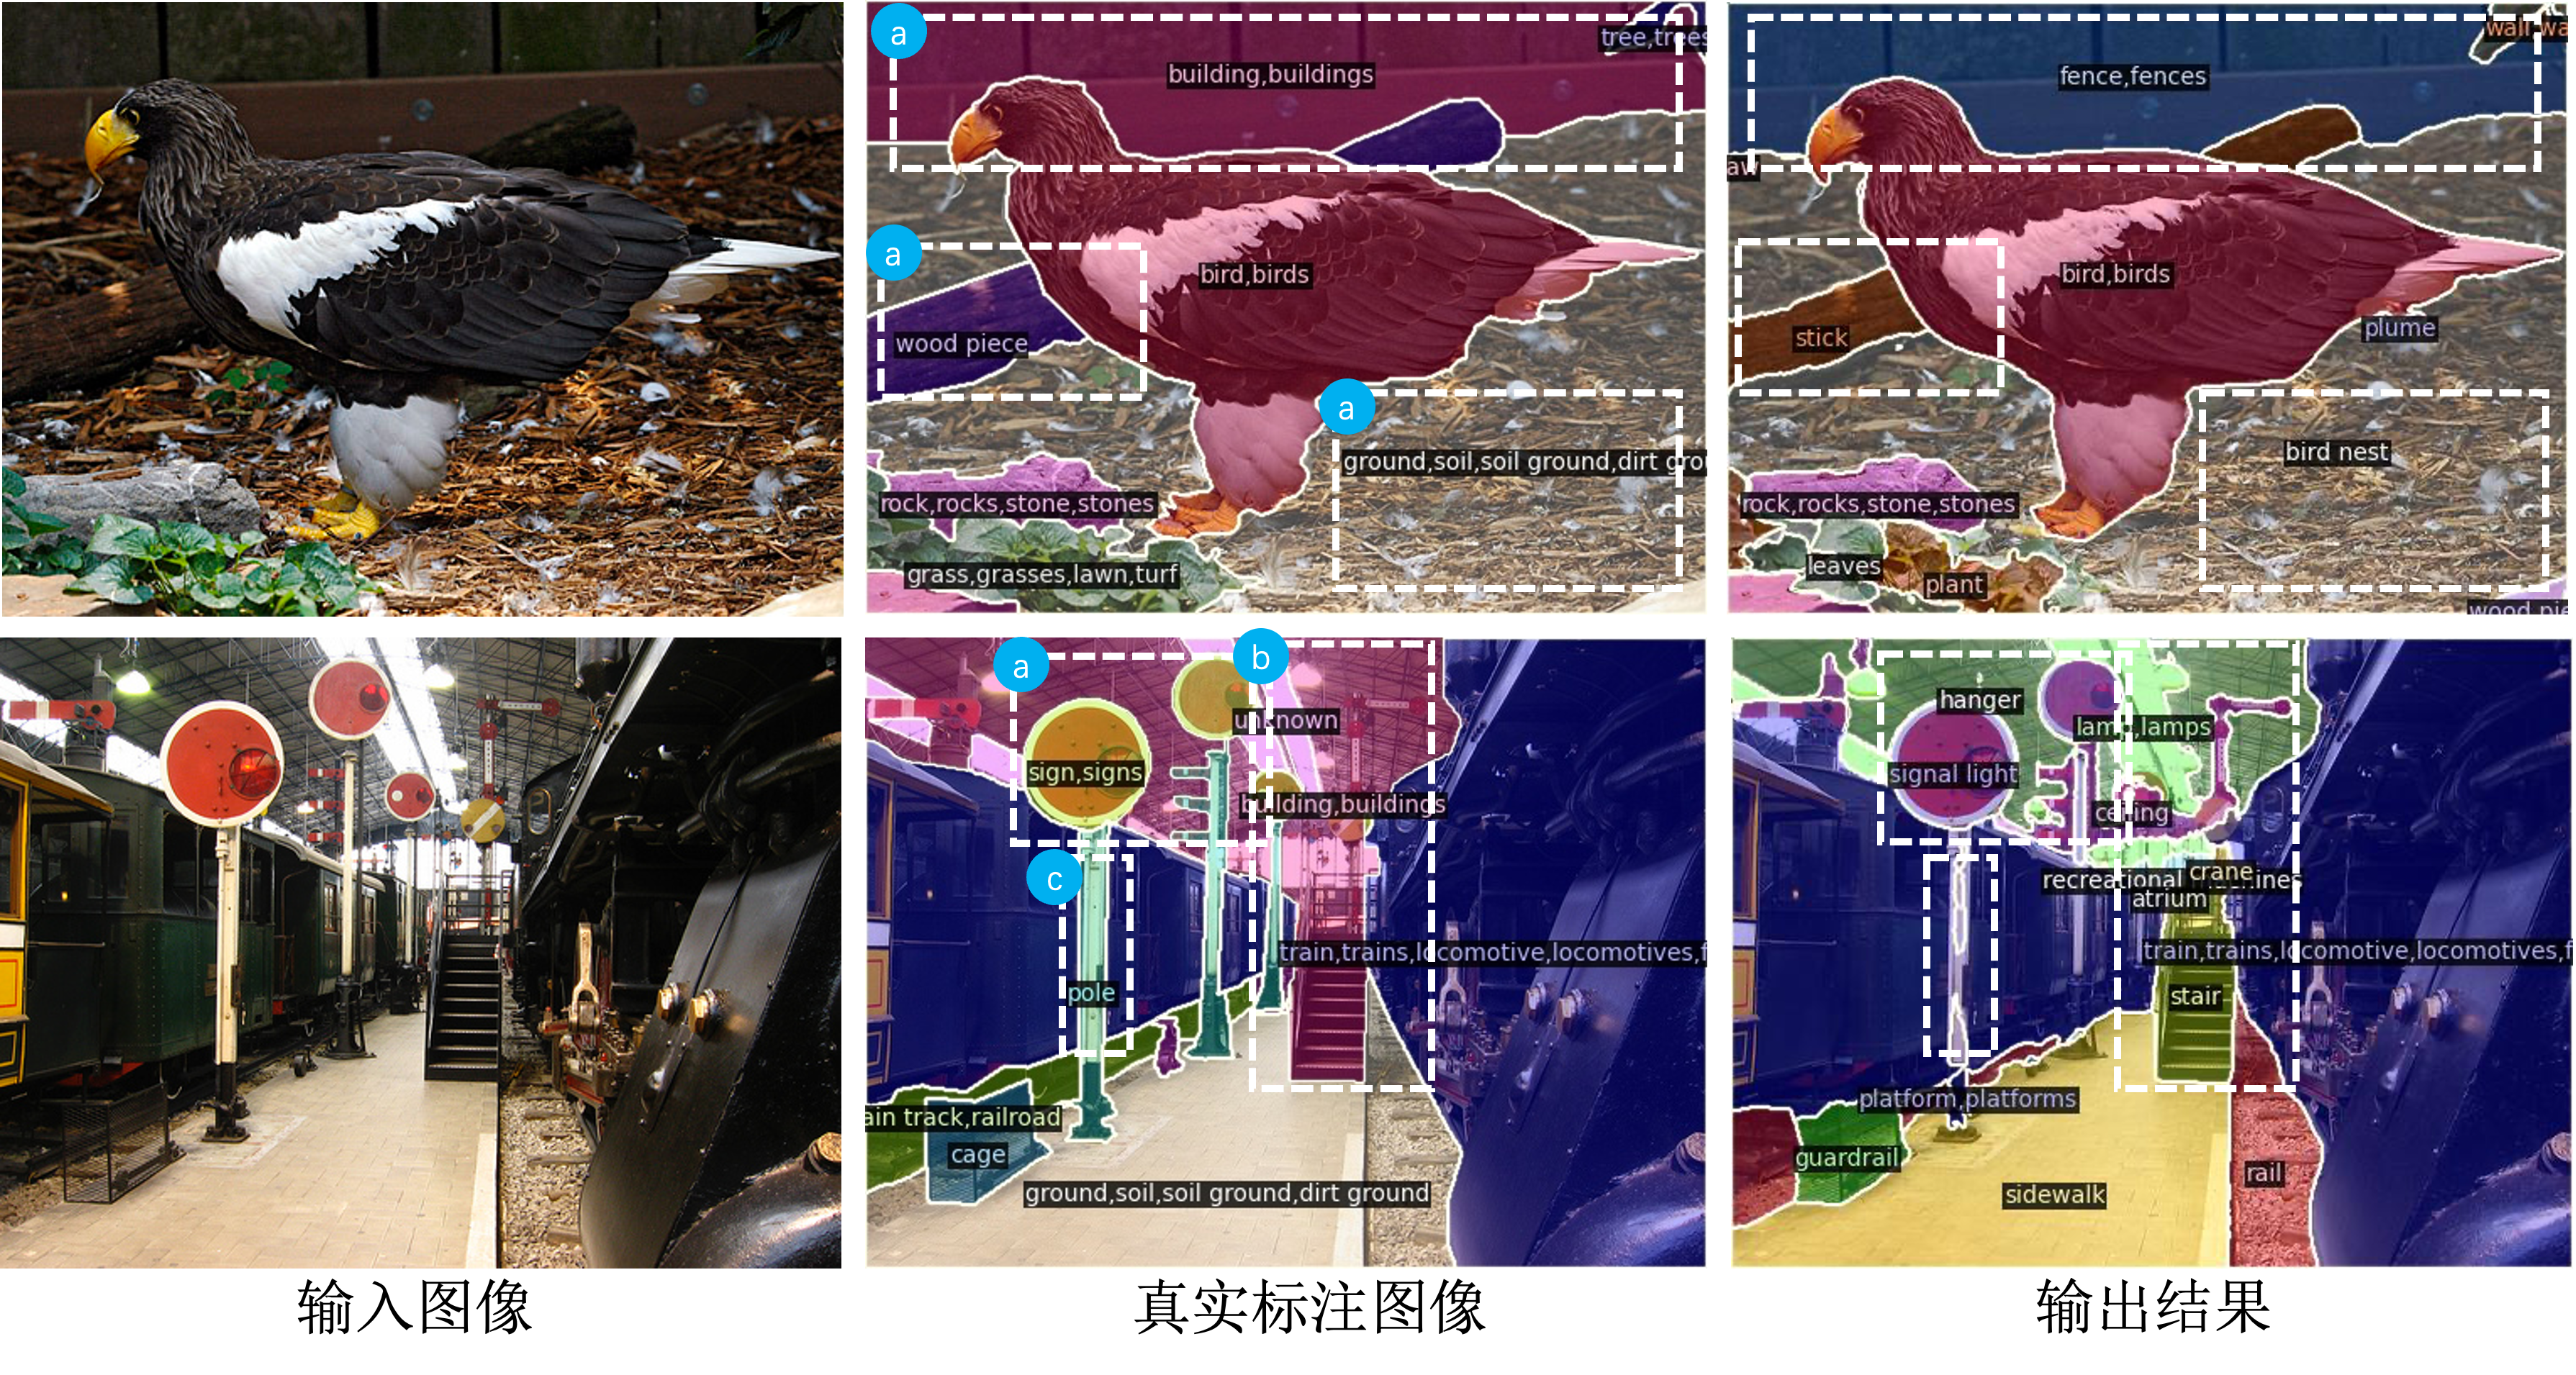
\includegraphics[width=0.85\textwidth]{figures/cmpf/fail_case.png}
%     \bicaption[fig:failure_case]{}{PC-459数据集上的典型失败案例：(a) 语义歧义；(b) 粒度不匹配；(c) 模糊边界}{Fig.}{Failure case examples on PC-459: (a) semantic ambiguity; (b) granularity mismatch; (c) ambiguous boundaries}
% \end{figure}

\FloatBarrier
\noindent\textbf{(4)推理速度与参数量对比}
\begin{table*}[!htbp]\centering
    \bicaption[tab:speed_cmpf]{}{CMPF与FC-CLIP的推理速度与参数量对比（单卡A100）}{Table}{Inference speed and parameter analysis}
    \vspace{0.5em}\centering\wuhao
    % \setlength{\tabcolsep}{2pt}
    % \resizebox{.5\textwidth}{!}{
        \begin{tabular}{lcccccc}
            \toprule
            \multirow{2}{*}{方法} & \multicolumn{2}{c}{ADE20K} & \multicolumn{2}{c}{A-847} & \multicolumn{2}{c}{参数 (M)} \\
            \cline{2-7}
             & PQ & FPS & PQ & FPS & 冻结 & 可训练 \\
            \midrule
            FC-CLIP~\cite{yu2023convolutions} & 25.1 & 2.7 & 14.0 & 3.1 & 200.0 & 21.0 \\
            SCAN~\cite{liu2024open} & -- & -- & 14.0 & 0.9 & 731.6 & 158.7 \\
            EOV-Seg~\cite{niu2025eov} & 24.5 & 11.6 & 12.8 & 11.8 & 203.7 & 21.8 \\
            \textbf{CMPF} & \textbf{25.9} & 2.2 & \textbf{14.4} & 2.9 & 293.5 & 26.5 \\
            \bottomrule
        \end{tabular}
        % }
\end{table*}


表~\ref{tab:speed_cmpf}给出了CMPF与同类CLIP基方法的推理速度与参数量对比。CMPF与FC-CLIP和SCAN的推理速度相当，额外引入的参数量带来了明显的精度提升，体现了良好的精度—效率权衡。

% \FloatBarrier

\section{本章小结}

本章围绕开放词汇分割中视觉—语言模型掩码质量不足的问题，沿训练期融合与推理期集成两个角度展开治理。训练期融合通过查询注入与特征注入两类轻量模块，在 Transformer 解码器内部实现分割基础模型的空间定位先验与视觉—语言模型的开放词汇语义先验的深度融合，且全程保持两个基础模型参数冻结；推理期集成通过类别与掩码的两阶段策略融合分割基础模型的零样本掩码预测，专门用于提升未见类别的分割质量。消融分析表明训练期特征融合是性能提升的主要驱动力，推理期掩码集成在其基础上提供互补增益。八个基准上的实验验证了方法在数据效率与泛化能力上的优势。

% Local Variables:% Local Variables:
% TeX-master: "../thesis"
% TeX-engine: xetex
% End:
